%Este documento es una plantilla del desarrolo de una tesis, espero pueda ser de apoyo a más
%estudiantes, cualquier objeto es este código puede ser tomado y reproducido en su parcualidad o 
% totalidad. Fuego a los derechos de autor

%Correo: Chavasalvador.jns@gmail.com

\documentclass[12pt]{book} % tamaño de letra, usamos por defecto la fuente de latex
\usepackage{graphicx} % paqueteria para incluir imagenes
\usepackage{longtable,multirow,booktabs} %formato para incluir tablas
\usepackage{caption} % para referencias
\usepackage[spanish,USenglish,es-tabla]{babel} % alterna inglés y español en la escritura
\usepackage[hidelinks]{hyperref} %elimina las casillas rojas en los hiperlinks
\usepackage{float} %aquete para mejorar la posición de flotantes
\setlength{\parskip}{1em} %
\usepackage[utf8]{inputenc}
\usepackage{fancyhdr}
\usepackage{lastpage}
\usepackage{amssymb} 
\usepackage{emptypage}
\usepackage{titlesec}
\usepackage{amsmath} 
\usepackage{subfigure}
\usepackage[papersize={216mm,279mm},lmargin=3cm,rmargin=2cm,top=2cm,bottom=2cm]{geometry}
%geometry define tamaño de papel para impresión así como el tamaño de los margenes
\usepackage{listings}
\titleformat{\chapter}[frame]{\normalfont}{\filcenter \small \ CAPÍTULO \  \thechapter \ }{7pt}{\Large\bfseries\filcenter} %defenimos el encabezado para los capitulos

\titleformat{\section}[display]
{}{\filcenter\bfseries Sección
\thesection.}{0pt}{\titlerule[1pt]
\itshape\fillast}[{\titlerule[1pt]}]

\setcounter{secnumdepth}{4}

\begin{document}

%cambiamos de inglés a español algunos comandos
\newtheorem{theorem}{Teorema}
\renewcommand{\contentsname}{Índice general}
\renewcommand{\listfigurename}{Índice de figuras}
\renewcommand{\listtablename}{Índice de tablas}
\renewcommand{\partname}{Parte}
\renewcommand{\appendixname}{Apéndice}
\renewcommand{\figurename}{Figura}
\renewcommand{\tablename}{Tabla}
\renewcommand{\chaptername}{Capítulo} 
\renewcommand{\bibname}{Bibliografía} 

\pagestyle{fancy}
\fancyhead{} % clear all header fields
\renewcommand{\headrulewidth}{0.0mm}
\lfoot{} 
\cfoot{\thepage} 
\rfoot{}

\thispagestyle{empty} % no numeramos la pagina

\begin{minipage}{.25\textwidth}
  \flushleft
  \center{
\includegraphics[scale=.07]{unam.png}}

  \vspace{20pt}

  \center{
    \rule{.5pt}{.6\textheight}
    \hspace{7pt}
    \rule{2pt}{.6\textheight}
    \hspace{7pt}
    \rule{.5pt}{.6\textheight}
  } \\

  \center{
\includegraphics[scale=.15]{FI.png}}
\end{minipage}
\begin{minipage}{.7\textwidth}
\flushright

\center{

  \center{
    \LARGE{U}\large{NIVERSIDAD} \LARGE{N}\large{ACIONAL} 
    \LARGE{A}\large{UTÓNOMA} \\[10pt]
    \large{DE} 
    \LARGE{M}\large{ÉXICO} 
  } \\
  \rule{\textwidth}{2pt}
  \\
  \hrulefill\\[.5cm]
  
  \LARGE{F}\large{ACULTAD DE } \LARGE{I}\large{NGENIERÍA}\\[1cm]

  \large{{\bf{
Diseño de Robot Asistente para Hospitales}}}\\[2cm]

  \huge{
T \hspace{1cm} E \hspace{1cm} S \hspace{1cm} I \hspace{1cm} S  }\\[1cm]

  \large{PARA OBTENER EL TÍTULO DE}\\[1cm]

  \large{
Ingeniero Eléctrico Electrónico}\\[1cm]

  \large{PRESENTA:}\\[1cm]

  \large{ \textbf{García Martínez Alan}
   }\\[1cm]

  \large{
TUTOR  }\\[1cm]

  \large{
Dr. Víctor Manuel Lomas Barrié}
}\\[1cm]

  \large{
México, CDMX, Coyoacán, C.U. \hspace{3cm} 2022   
}

\end{minipage}

\newpage

\pagenumbering{Roman} 

\clearpage\hbox{}\thispagestyle{empty}\newpage

Jurado asignado:

\vspace{2cm}

%Presidente.       \hspace{1.9cm} Dr. Armando Marín Becerra

%Vocal.            \hspace{2.8cm} Dr. Luis Emilio Orgaz Baqué

%Secretario.	     \hspace{2cm} Dr. José Enrique Barquera Lozada

%Primer Suplente.  \hspace{0.85cm} M en C. Margarita Chávez Martínez

%Segundo Suplente.  \hspace{0.6cm} Dr. Jorge Martin del Campo Ramírez

\vspace{2cm}
Sitio en donde se desarrolló el tema:

Instituto de Investigaciones de Matemáticas Aplicadas y en Sistemas.

Laboratorio de Róbotica.

Ciudad Universitaria.

Universidad Nacional Autónoma de México.

\vspace{2cm}

\rule{7.5cm}{0.3mm} 

Dr. Víctor Manuel Lomas Barrié

Asesor de Tesis 


%\vspace{2cm}
%\rule{7.5cm}{0.3mm} 
%Carlos Alberto Salvador Jiménez Rosas
%Sustentante

\newpage
\vspace{6cm}

Los resultados y avances de esta tesis, se presentaron en:

%\begin{itemize}
%	\item XXXV Simposio interno del Instituto de Química, 2018. Ciudad de México, Coyoacán. ``Estudio teórico topológico del flujo de corriente eléctrica en compuestos tipo $ML_4$". Modalidad cartel
	
%	\item Química y materiales en el siglo XXI. Future of science 2019. Ciudad de México, Coyoacán. ``Theoretical-topological study of electric current flow". Modalidad cartel
	
%	\item XXXVII Simposio interno del Instituto de Química, 2020. Ciudad de México, Coyoacán. ``Theoretical-topological study of electric current flow". Modalidad cartel
%\end{itemize}

\newpage

\clearpage\hbox{}\thispagestyle{empty}\newpage

\begin{center}
\huge{Agradecimientos}
\end{center}

\vspace{1cm}

Dedico mi esfuerzo y conocimiento a las personas que me han apoyado a lo largo de mi formación acádemica y formación profesional para ser la persona con la que me propuse ser un día.\\
Un Agradecimiento a mi madre quien me ha apoyado en multiples ocasiones para poder completar mi educación.\\
Un agradecimiento a mi Padre quien con su apoyo logre persistir a través de estos años para no desistir y lograr todas mis metas.


\begin{flushright}
\textit{Alan García Martínez \\
Álvaro Obregón Ciudad de México, 2022.
}
\end{flushright}

\newpage


\hspace{5cm}


\newpage %declaramosqueremos continuar la impresión en l siguiente página

\clearpage\hbox{}\thispagestyle{empty}\newpage

%para agregar algunas citas inclinadas a la izquierda o la dercha

\begin{flushright}
\textit{ Cada libro, cada tomo que ves, tiene alma. \\
El alma de quien lo escribió,\\
 y el alma de quienes lo leyeron y vivieron y soñaron con él \\ [0.5cm]
-La sombra del viento. Carlos Ruiz Zafón.}
\end{flushright}

\vspace{5cm}

\begin{flushleft}

%\end{flushleft}
\textit{ El futuro nunca lo vi,\\
se convirtió en ayer, \\
cuando intentaba alcanzarlo.\\[0.5cm]
-Esperanza. José Emilio Pacheco.}
\end{flushleft}

\vspace{5cm}

%\begin{flushright}
%\textit{Aquí son hermosas cuatro florecitas, \\
%su cuerpo aparece como espejo radiante, \\
%sus hojas son bella aurora, \\
%tus raíces son el cordón umbilical, \\
%tus espigas son el plumaje y el canto de las aves, \\
%tu fruto es mi sangre, es mi cuerpo, \\
%porque tú me provees de alimento, \\
%¿Por qué estoy vivo? ¡Por qué estás aquí!\\[0.5cm]
%-Poema al maíz.}
%\end{flushright}

\tableofcontents % indice de contenidos
\addcontentsline{toc}{chapter}{Índice general}

\cleardoublepage
\addcontentsline{toc}{chapter}{Índice de figuras} % para que aparezca en el indice de contenidos
\listoffigures % indice de figuras

\cleardoublepage
\addcontentsline{toc}{chapter}{Índice de tablas} % para que aparezca en el indice de contenidos
\listoftables % indice de tablas

% encabezados
\lhead[]{CAPÍTULO \ \thechapter.\ \rightmark} %impares
\chead[]{}
\rhead[CAPÍTULO \ \thechapter. \ \leftmark]{} %pares 
\renewcommand{\headrulewidth}{0.5pt}

% pie de pagina
\lfoot[]{P\'gina \thepage \hspace{1pt} de \pageref{LastPage}}
\cfoot[]{}
\rfoot[P\'agina \thepage \hspace{1pt} de \pageref{LastPage}]{}
\renewcommand{\footrulewidth}{0.5pt}

% primera pagina de un capitulo
\fancypagestyle{plain}{
\fancyhead[L]{}
\fancyhead[C]{}
\fancyhead[R]{}
\fancyfoot[L]{}
\fancyfoot[C]{}
\fancyfoot[R]{}
\renewcommand{\headrulewidth}{0pt}
\renewcommand{\footrulewidth}{0pt}
}

\pagestyle{fancy}

\chapter{Resumen}
	\label{cap.intro}

\markboth{RESUMEN}{RESUMEN}

\pagenumbering{arabic}
\setcounter{page}{1}

Las necesidades de cubrir los servicios y productos han llevado a la sociedad a buscar nuevas formas de innovar y modernizar la logística para la producción de productos de todo tipo y colaborar en la participación de distintos servicios en favor de la sociedad moderna, consolidado por la industria 4.0 implicando consigo mayor productividad y eficiencia entre otras ventajas como la reducción de márgenes de error y procesos precisos y eficientes reduciendo tiempos de producción y costos de operación.
\\
Con lo anterior en mente se implementó el diseño de control de un robot móvil haciendo uso de multiples herramientas matamáticas y el diseño de algoritmo para la navegación adecuada con el fin de poder ser implementado en los hospitales para la asistencia a personal médico profesional para lograr optimizar multiples procesos.

\chapter{Antecedentes}
	\markboth{ANTECEDENTES}{ANTECEDENTES}
\begin{flushright}
\textit{“La róbotica se define como una ciencia que reúne diferentes campos tecnológicos, con el principal objetivo de diseñar máquinas robotizadas capaces de realizar diferentes tareas automatizadas en función de la capacidad de su software.
\\[0.1cm]
-EDS Robotics.}
\end{flushright}

\begin{flushright}
\textit{“Un robot es una máquina capaz de extraer información de su ambiente y usa el conocimiento acerca de su mundo para moverse de manera segura para realizar un propósito especifico.
\\[0.1cm]
-1942, Isaac Asimov.}
\end{flushright}
	\section{Planteamiento del problema }
	\lhead[]{\thesection \ Planteamiento del problema.}
La pandemia del COVID-19 durante el año 2019 nos planteó una nueva visión sobre la situación sanitaria que implicó la alta tasa de los contagios que se suscitaron durante los primeros meses de la pandemia, por lo que al tiempo de realizar analisis y estudios en las áreas encargadas para atender el COVID-19 se propuso utilizar robots para la asistencia médica en áreas específicas y automatizar tareas específicas dentro de los hospitales con el propósito de reducir el contagio entre el personal médico y los pacientes, sin embargó se requieren proponer nuevos diseños y protocolos para los robots dentro de los hospitales para poder atender en capacidad diferentes situaciones sanitarias que se puedan presentar más adelante para mejorar la atención médica.
\newpage
	\section{Importancia de la róbotica para la sociedad actual.}
	\lhead[]{\thesection \ Importancia de la róbotica para la sociedad actual.}

	Los constantes avances de la tecnología generan cambios en nuestra sociedad en la forma en la que llevamos a cabo nuestras actividades cotidianas, facilitando tareas que solían ser más complicadas en años anteriore. La busqueda por optimizar y automatizar las tareas han llevado la busqueda la inovación y evolución en los diferentes métodos de software y hardware para satisfacer la necesidad de realizar tareas automatizadas en las últimas decadas.\\
	La róbotica no solo ha ayudado a mejorar los tiempos de producción continua y de calidad para industrias de todo tipo como por ejemplo la automotriz, farmaceutica, constructora entre muchas otras industrias que emplean los brazos róboticos para realizar tareas complejas.\\
	Sin embargó no solo en las industrias han sido beneficiadas por los avances en róbotica, ya que dentro del área médica los brazos róboticos han sido una herramienta de bastante demanda debido a la capacidad de llevar acabo complejas operaciones en pacientes. Nos referimos a sistemas de brazos róboticos como el modelo Zeus y el modelo Davinci que tomaron mucha relevancia en hospitales para realizar diferentes operaciones.\\
En lo que respecta a el área médica y en particular la cirugía robótica, se han tenido progresivos avances enfocados a la robótica utilizadas en las cirugías que presentan una mayor complicación de realizar, siendo considerada como por muchos autores como el futuro en las cirugías ya que su desarrollo ha sido rápido y ha demostrado poseer numerosas ventajas que ayudan a la mejora de las técnicas quirúrgicas gracias a el desarrollo de la industria 4.0 y el IOT.\\
De igual manera gracias a la cirugía robótica se han producido
cambios en la práctica y en la enseñanza de la cirugía que cada vez son más comunes, a continuación, exploraremos técnicas y conceptos de la cirugía robótica.	\\
	
\chapter{Objetivos e hipótesis} \label{cap.Objetivos} 
 \markboth{OBJETIVOS E HIPÓTESIS}{OBJETIVOS E HIPÓTESIS}
 
\section{Objetivo General}
\lhead[]{\thesection \ Objetivo General} 
Diseñar un sistema de control para la navegación de un robot móvil sobre una plataforma omnidireccional que cumpla con funciones de asistente enfermero para hospitales designados como apoyo y atención a pacientes de COVID-19.

\section{Objetivos Específicos.}
\lhead[]{\thesection \ Objetivos Específicos.}
\subsection{Caracterización de un robot móvil con diseño omnidireccional.}
\lhead[]{\thesection \ Caracterización de un robot móvil con diseño omnidireccional.}
Se busca incorporar en la navegación de un robot móvil a partir de 4 ruedas mecanum para la navegación del robot asistente para lograr optimizar procesos de navegación dentro de áreas médicas especificas.


\subsection{Diseño del tren motriz para navegación del robot.}
\lhead[]{\thesection \ Diseño del tren motriz para navegación del robot.}
Se propondra un diseño en base a un circuito considerando aspectos como alimentación, protección contra picos de corriente y control del movimiento del robot móvil en base a un algoritmo de navegación y un esquema de conexiones eléctronicas.

\subsection{Diseño del algoritmo para la navegación del robot móvil.}
\lhead[]{\thesection \ Diseño del algoritmo para la navegación del robot móvil.}

Se busca diseñar e implementar con la eléctronica un algoritmo de programación en lenguade de C para el microcontrolador Raspberry PI Pico para controlar el tren motriz del robot.

\subsection{Implementación de tópicos de ROS para el robot móvil.}
\lhead[]{\thesection \ Implementación de tópicos de ROS para el robot móvil.}
Se planteara implementar en conjunto con las herramientas proporcionadas por ROS2 org en uso de la distribución de ROS2 Foxy, tópicos para la comunicación serial entre la Raspberry PI4 y la raspberry Pi Pico.


\chapter{Marco teórico} \label{cap.marco_teo}
 \markboth{MARCO TEÓRICO}{MARCO TEÓRICO}
 
	\section{Sistema motriz de robots móviles}
		\lhead[]{\thesection \ Sistema motriz de robots móviles}
		
	\subsection{Rueda Mecanum}
		\lhead[]{\thesection \ Rueda Mecanum}
La rueda omnidireccional o rueda Mecanum a diferencia de un rueda normal tiene la caracteristica de tener un cubo de rueda y un rodillo. La función del cubo es ser el soporte principal de la rueda mientras que el rodillo es un tambor montado en el tubo como se muestra en la figura 4.1.\\
\begin{figure}[H]
\centering
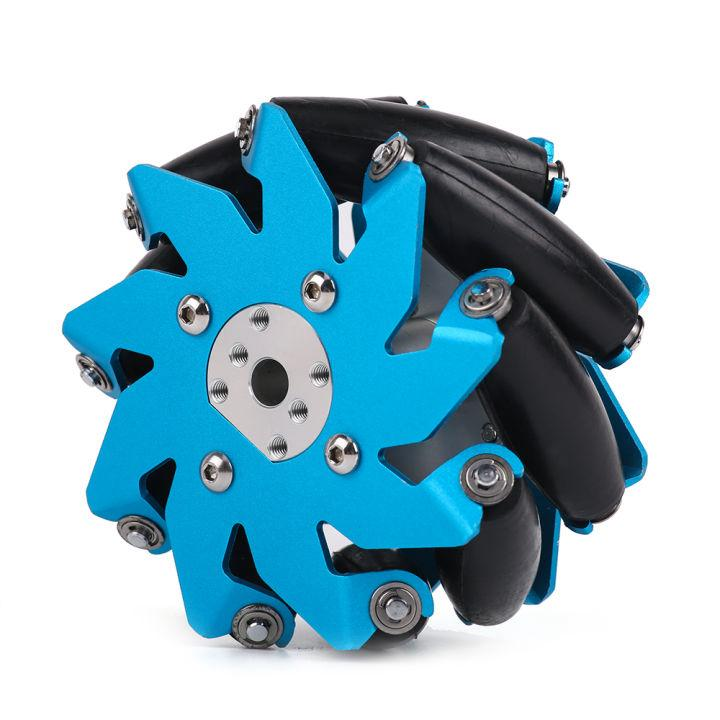
\includegraphics[scale=0.3]{Mecanum.jpg} 
\caption{Rueda Mecanum} 

\end{figure}

El eje del cubo de la rueda omnidireccional y el eje del rodillo son perpendiculares entre sí, mientras que el eje del cubo de la rueda Mecanum y el eje del rodillo están en un ángulo de 45 °.\\
Esto permite que las ruedas se muevan en dos direcciones y se muevan holonómicamente, asegurando que puedan moverse instantáneamente en cualquier dirección.\\

\begin{figure}[H]
\centering
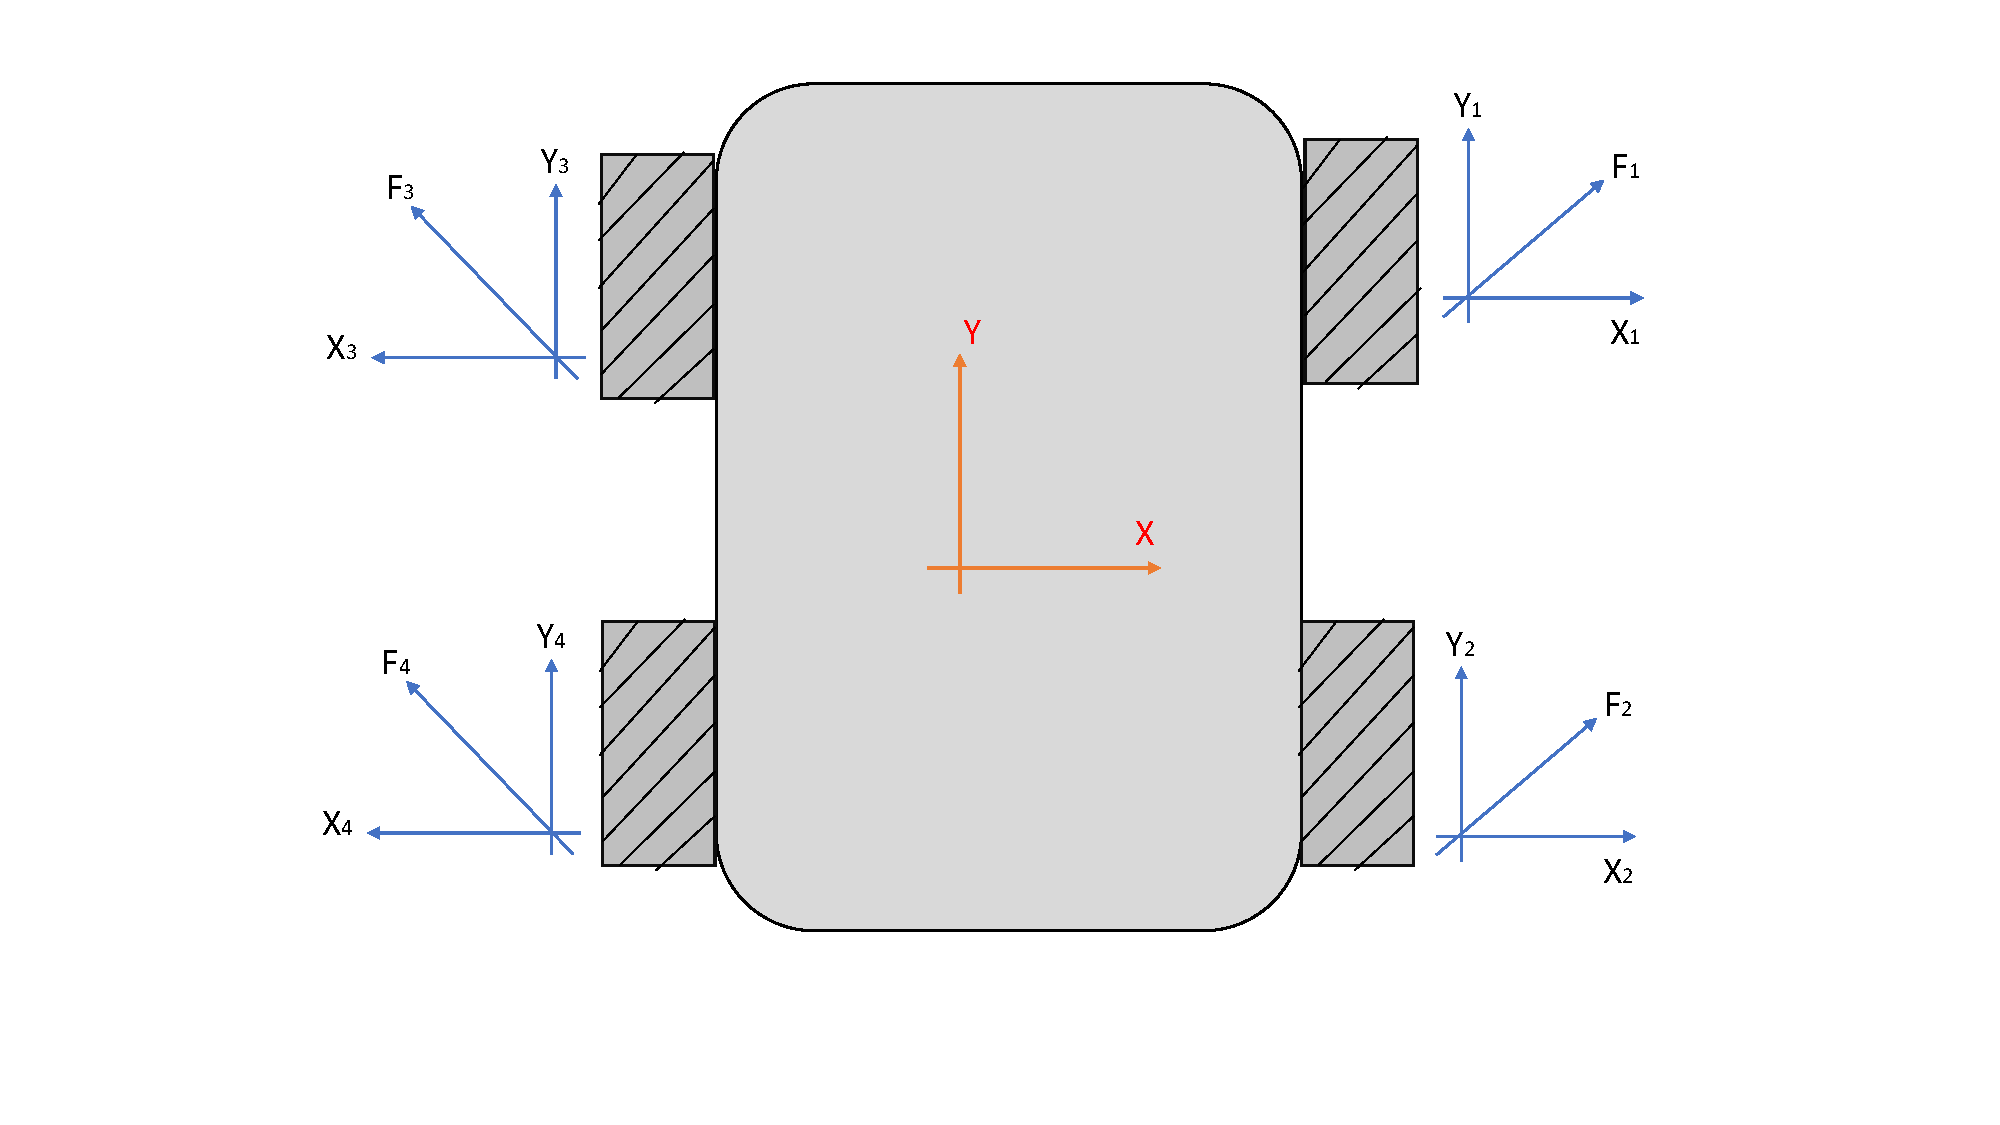
\includegraphics[scale=0.4]{Direcciones.pdf} 
\caption{Direcciones para una plataformar compuesta de 4 ruedas mecanum.} 
\end{figure}
Como se observa en la figura 4.2, al tener una direccion de giro en la rueda, por ejemplo en el eje "Y", tendremos a la para una componente horizontal sobre un eje "X", y en consecuencia también tendremos una fuerza resultante en un angulo a 45°.

	\subsection{Movimiento Omnidireccional de un robot móvil}
		\lhead[]{\thesection \ Movimiento Omnidireccional de un robot móvil}

El movimiento omnidireccional en la aplicación de los robots móviles es cada vez más común debido a la gran versatilidad y ventajas que propone este sistema de movimientos para los robots móviles representa en una mayor libertad de movimiento para desplazarse.\\Como se detalló anteriormente, el movimiento omnidireccional se debe a el uso de 4 ruedas mecanum pueden viajar en cualquier dirección desde cualquier ángulo sin girar de antemano permitiendo desplazamientos horizonales, verticales, diagonales y girar sobre un eje de referencia. Como se muestra en la Figura 4.2 tendremos 10 principales formas de movimiento.\\

\begin{figure}[H]
\centering
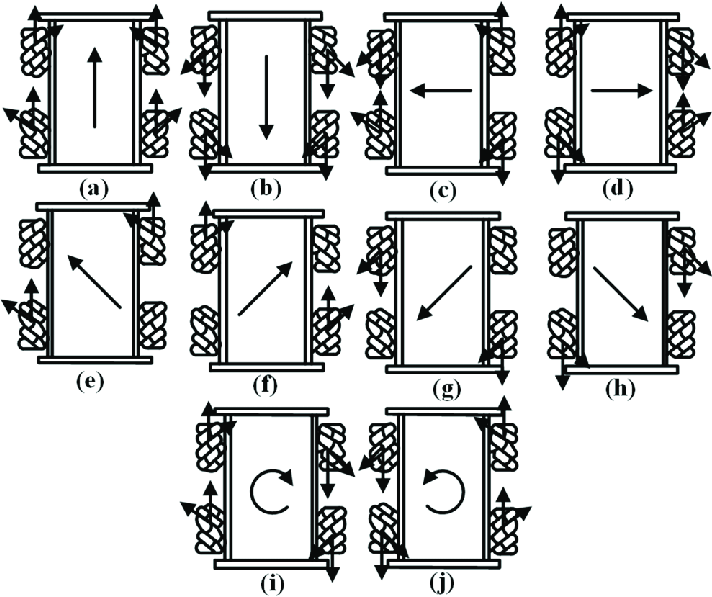
\includegraphics[scale=0.4]{Fig-5-Top-view-of-turning-principle-of-Mecanum-wheel.png} 
\caption{Tipos de movimientos con una plataforma omnidireccional. Imagen obtenida de: www.researchgate.net} 
\end{figure}

De la Figura 4.2 a. Tenemos un movimiento hacia delante, el cual consiste principalmente en tener todas las ruedas hacia una misma dirección.\\
De la Figura 4.2 b. Tenemos un movimiento de reversa, con la diferencia de que es en sentido contrario al sentido del movimiento delantero.\\
De la Figura 4.2 c y d. Tenemos un movimiento horizontal hacia el lado izquierdo. Los movimientos horizontales tienen la característica de que los sentidos de giro estan determinados por que las ruedas correspondientes al lado izquierdo y derecho deben girar en sentidos contrarios al modo horario y antihorario deseados. Es decir que en este caso tendremos las ruedas del lado izquierdo girando de manera que ambas direcciones coincidan en un vector de movimiento resultante a la dirección izquierda y derecha respectivamente.\\
De la Figura 4.2 e, f, g, h. Son movimientos con vectores resultantes en diagonal, resultado de tener funcionando unicamente dos ruedas omnidireccionales en sentido diagonal hacia una misma dirección, para obtener en cada caso el desplazamiento de movimiento deseado.\\
De la Figura 4.2 i y j. Tenemos un movimiento de giro en 360° para la plataforma del robot omnidireccional, para lograr este sentido de giro las ruedas de lado izquierdo deben seguir una misma dirección de avance, mientras que por el contrario las ruedas del lado derecho deben ir en dirección contraria para lograr este giro de 360°.

Para la caracterización de los movimientos anteriormente mencionados tomaremos como referencia el movimiento y el sentido de giro que deben tener.\\
\begin{table}[t]
\begin{center}
\begin{tabular}{| p{4cm} | p{3cm} | p{3cm} | p{3cm}  | p{3cm} |} 
	
	\hline
	Movimiento & Rueda 1 & Rueda 2 & Rueda 3 & Rueda 4\\
	\hline
	ALTO & Sin movimiento & Sin movimiento & Sin movimiento & Sin movimiento\\
	\hline
	ADELANTE & Sentido Horario & Sentido Horario & Sentido Horario & Sentido Horario\\
	\hline
	ATRAS & Sentido Anti horario & Sentido Anti horario & Sentido Anti horario & Sentido Anti horario\\
	\hline
	DERECHA & Sentido Horario & Sentido Anti Horario & Sentido Anti horario & Sentido Horario\\
	\hline
	IZQUIERDA & Sentido Anti horario & Sentido Horario & Sentido Horario & Sentido Anti horario\\
	\hline
	DIAGONAL D1 & Sentido Horario & Sin movimiento & Sin movimiento & Sentido Horario\\
	\hline
	DIAGONAL D2 & Sin movimiento & Sentido Anti horario & Sentido Anti horario & Sin movimiento\\
	\hline
	DIAGONAL I1 & Sin movimiento & Sentido Horario & Sentido Horario & Sin movimiento\\
	\hline
	DIAGONAL I2 & Sin movimiento & Sentido Anti horario & Sentido Anti horario & Sin movimiento\\
	\hline
Giro en sentido anti horario & Sin Horario & Sentido Horario & Sentido Anti horario & Sentido Anti horario\\
	\hline
Giro en sentido horario & entido Anti horario & Sentido Anti horario & Sentido Anti Horario & Sentido Horario\\
	\hline
\end{tabular}
\caption{Caracterización de movimientos.}
\end{center}
\end{table}

\subsection{Driver controlador de motores de DC modelo Talon SR}
		\lhead[]{\thesection \ Driver controlador de motores de DC modelo Talon SR}
El driver controlador para motores de corriente directa modelo Talon SR, que se muestra en la siguiente figura. Es un dispositivo que controla la dirección de giro de los motores que utilizaremos para definir los movimientos de nuestro robot.\\
\begin{figure}[H]
	\begin{center}
	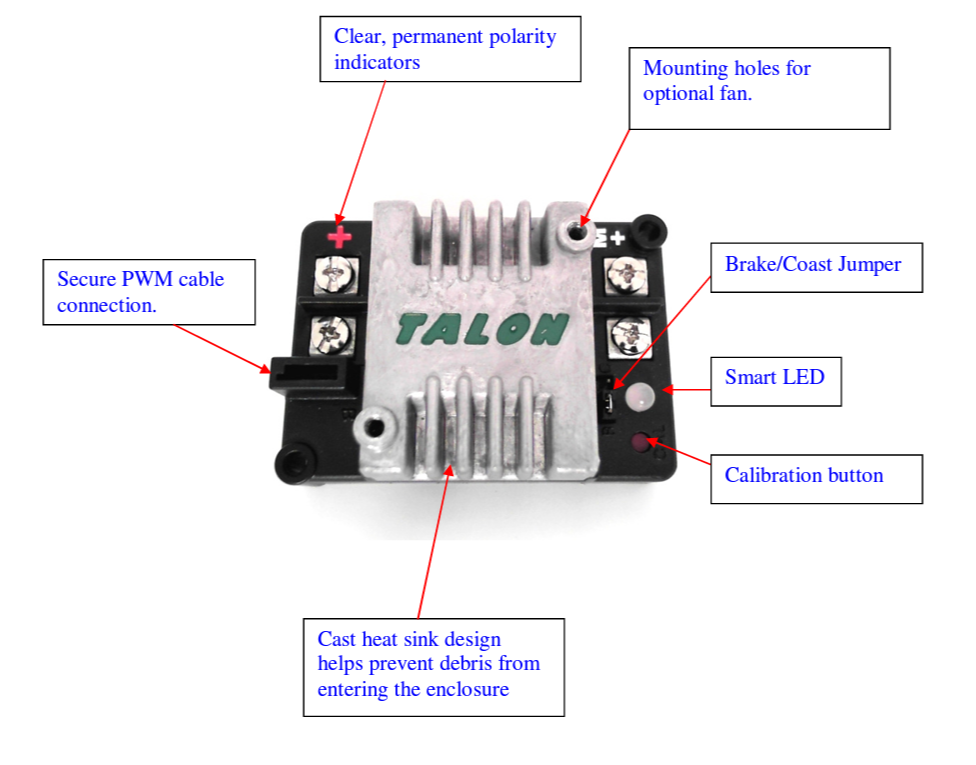
\includegraphics[width =16cm,height =7cm]{Talon.png}
	\caption{Driver controlador de motores Talon SR.} 
	\end{center}
\end{figure}
El funcionamiento de este dispositivo es controlar la velocidad y rotación de un motor de corriente directa mediante una señal modulada por ancho de pulsos o conocida como PWM para determinar la velocidad y sentido de giro del motor.\\
Como se observa en la figura 4.4, el talon principalmente tiene como caracteristicas una terminal de lado izquierdo con polaridad para alimentar el dispositivo con un rango de voltaje de 6 a 28 Volts. Tiene capacidad para soportar una corriente de hasta 36 Amperes.Tiene una terminal de 3 pines de los cuales tendremos una terminal con referencia a tierra y una para la señal PWM con la que controlaremos el dispositivo.\\
En el centro tenemos u disipador de temperatura al que se le puede adaptar un ventidalor. De lado derecho tenemos la terminal de salida donde se conecta a el motor de corriente directa. Tendremos un biled de dolor verde y rojo respectivamente para identificar el sentido de dirección de giro del motor. y una intermitencia de color naranja que indica que no esta actuando el motor, ya sea por la señal de modulación enviada o por que no recibe esta señal.\\
Adicionalmente este dispositivo puede ser calibrado para ser adaptable a un microcontrolador al que se desea ocupar. Sin embargó este dispositivo tiene la característica de necesitar un intervalo de 1-2 milisegundos.


\subsection{Motor DC modelo AM802-001A}
\lhead[]{\thesection \Motor DC modelo AM802-001A}		

\begin{figure}[H]
	\begin{center}
	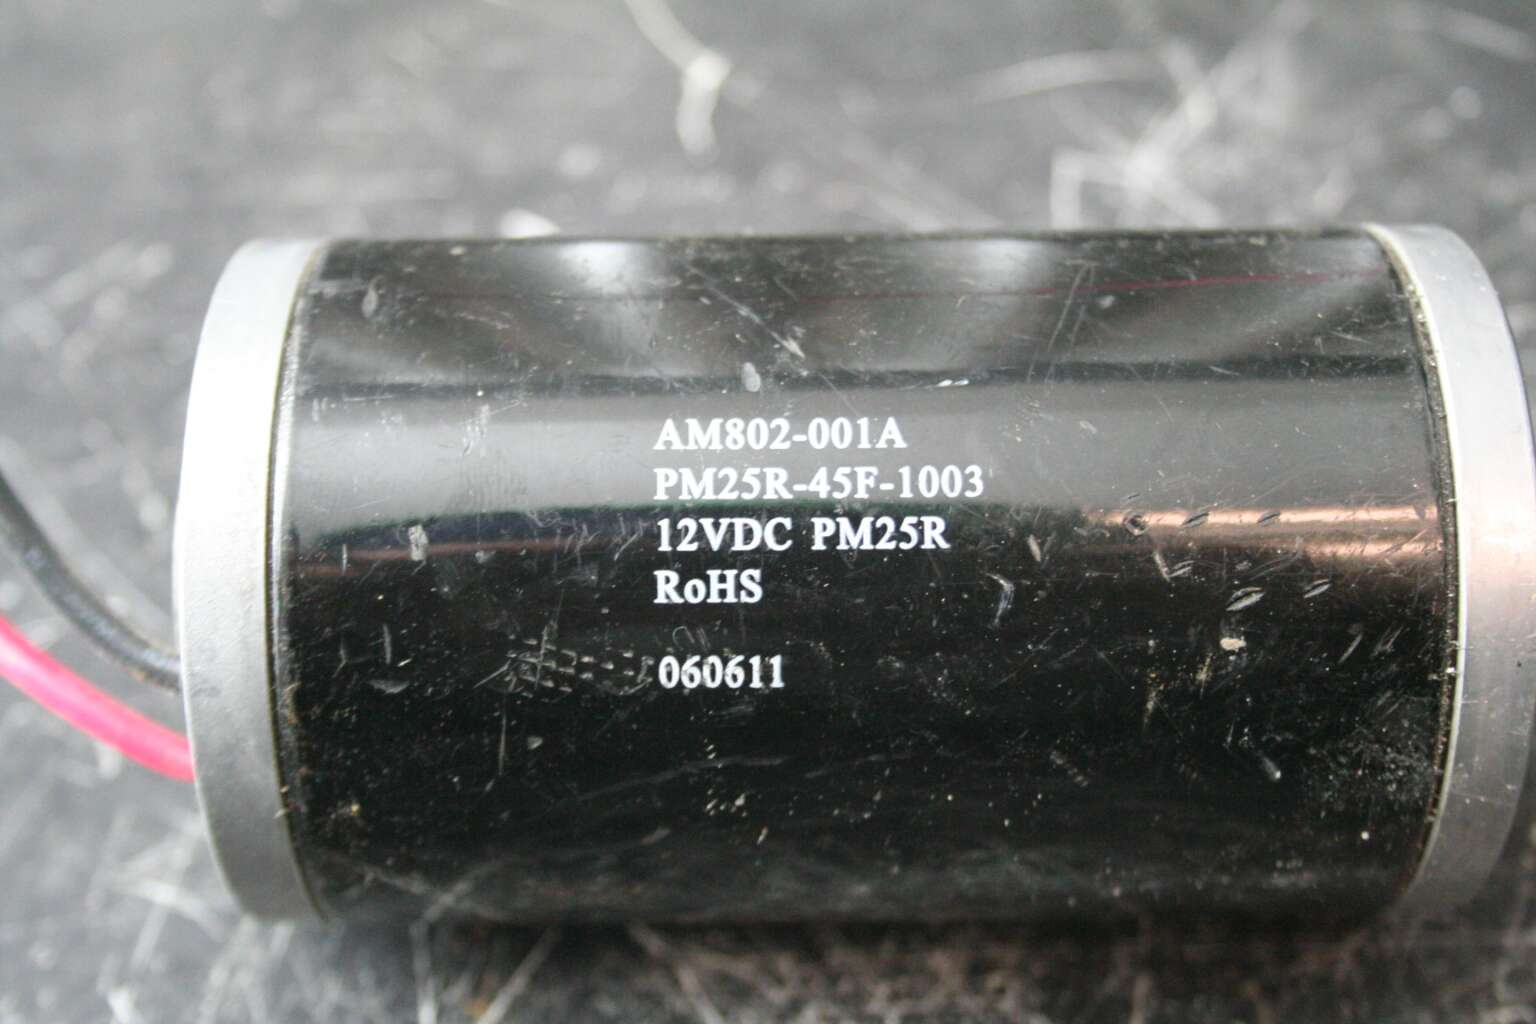
\includegraphics[scale=0.2]{AM801.jpg}
	\caption{Raspberry Pi Pico.} 
	\end{center}
	\end{figure}
	
El motor de corriente directa modelo AM802-001A, es un motor con las siguientes características.\\
- Voltaje nóminal de alimentación a 12 [V]\\
- 5310 RPM\\
- Capacidad de corriente de 133 [A]\\
- Corriente de arranque de 2.3 [A]\\
- Potencia máxima de 377 [W]\\

	\section{Microcontrolador Raspberry PI Pico}
		\lhead[]{\thesection \ Microcontrolador Raspberry PI Pico}
El dispositivo Raspberry Pi Pico es un microcontrolador basado en un chip RP2040, que brinda un alto rendimiento, bajo costo y facilidad de uso debido a que permite entornos de desarrollo en Micropython y en C/C++.\\
\begin{figure}[H]
	\begin{center}
	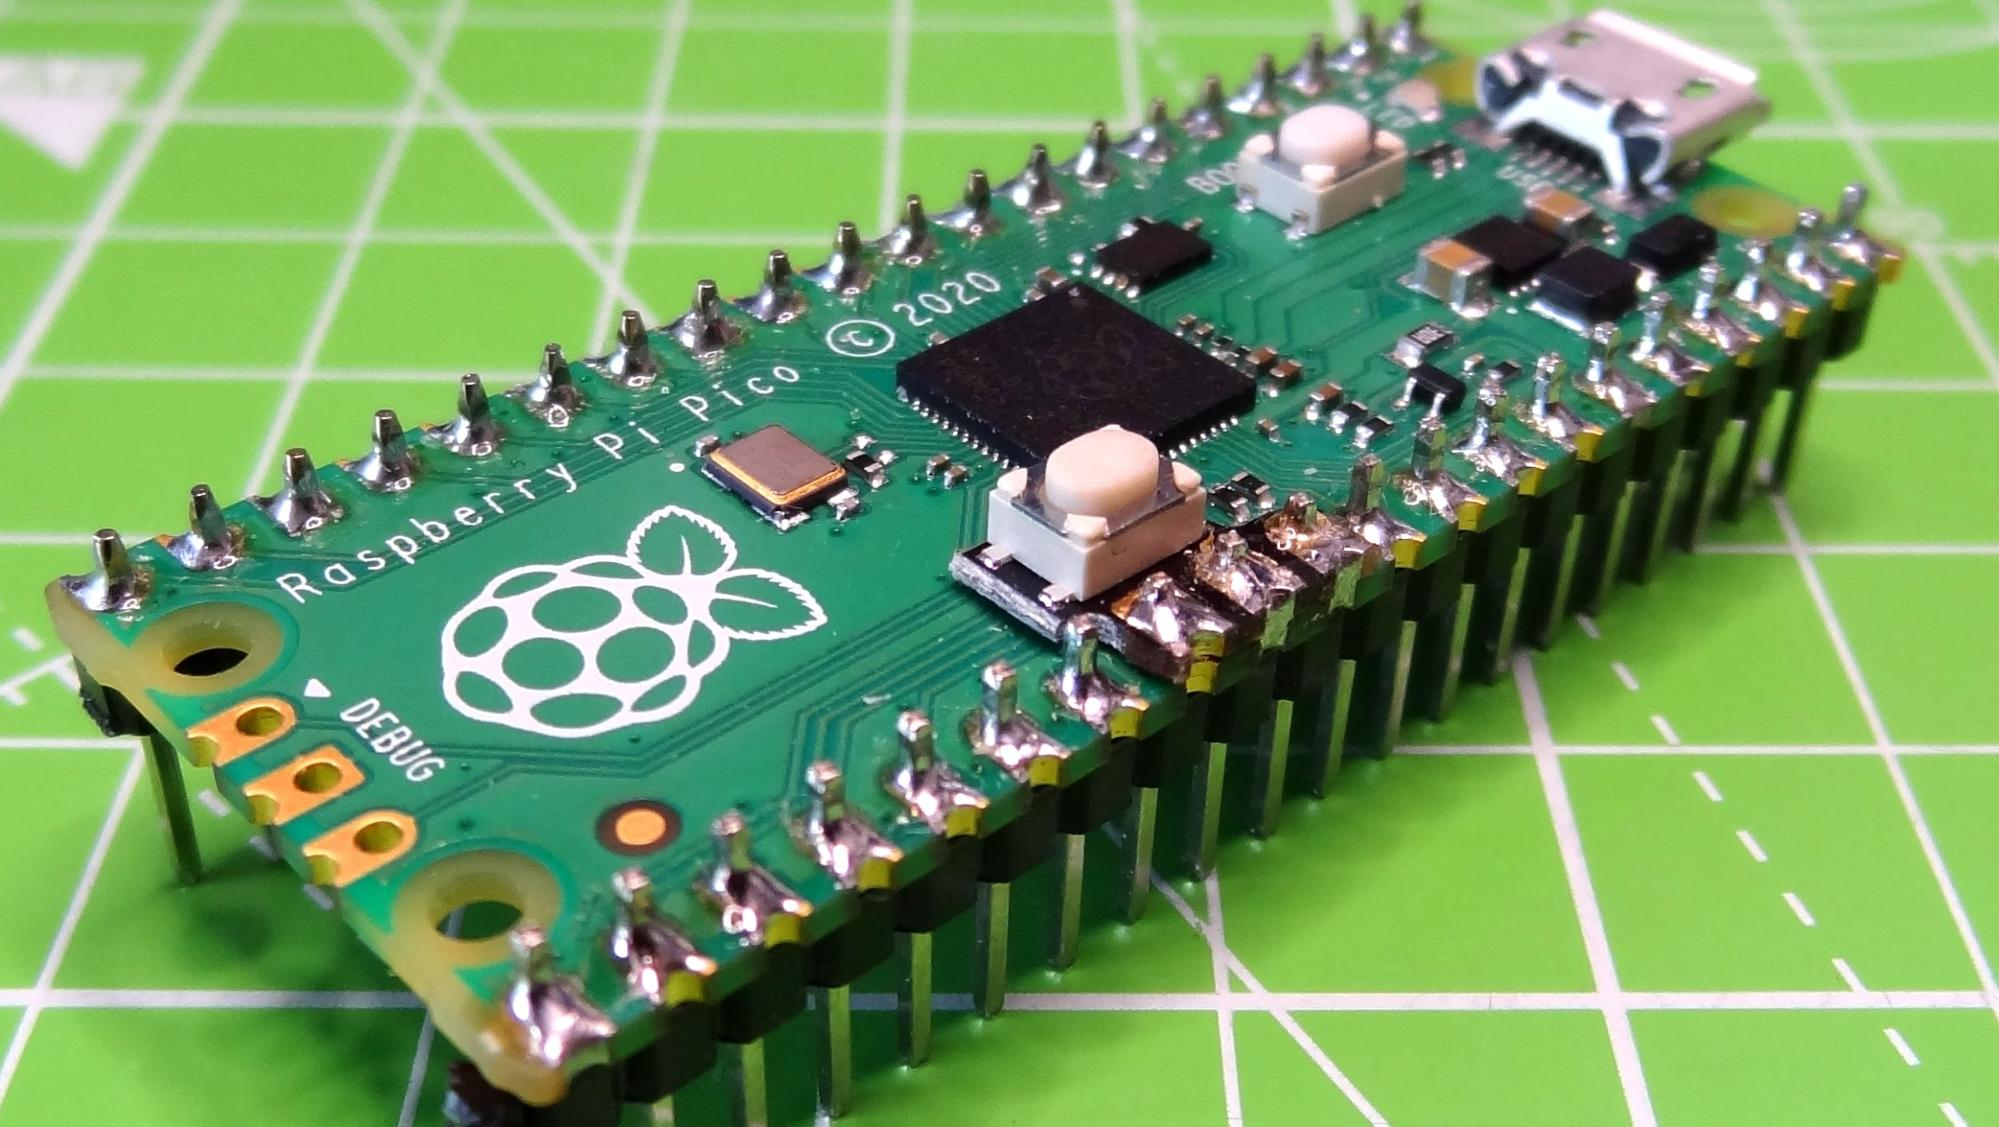
\includegraphics[scale=0.2]{Pico.jpg}
	\caption{Raspberry Pi Pico.} 
	\end{center}
	\end{figure}


Este dispositivo ademas de tener un costo relativamente bajo de 4 dolares, es bastante versital ya que tiene un total de 43 pines, los cuales se detallan en la siguiente figura.

	\begin{figure}[H]
	\begin{center}
	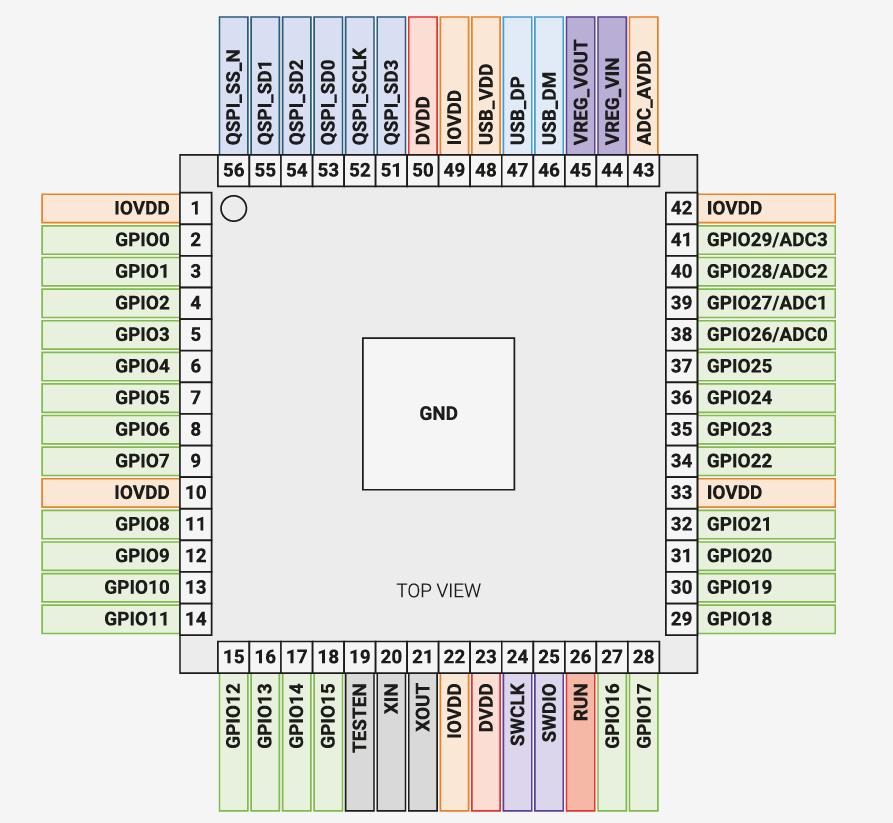
\includegraphics[scale=0.6]{RP2040.png}
	\caption{Driver controlador de motores Talon SR.} 
	\end{center}
	\end{figure}

La arquitectura físicamente en el controlador se detalla ahora en la siguiente figura.

	\begin{figure}[H]
	\begin{center}
	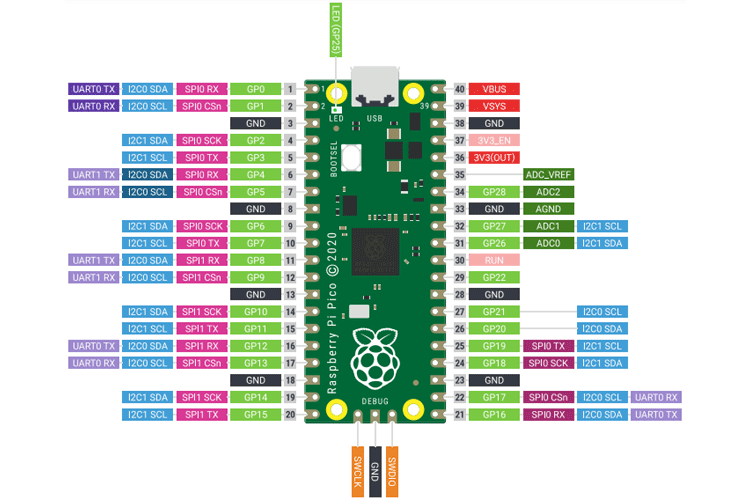
\includegraphics[scale=0.5]{Raspberry-Pi-Pico-Pinout.png}
	\caption{Driver controlador de motores Talon SR.} 
	\end{center}
	\end{figure}

	\section{Raspberry PI 4 MODEL B}
		\lhead[]{\thesection \ Raspberry PI 4 MODEL B}
La raspberry PI 4 MODEL B, es básicamente un dispositivo eléctronico que tiene la función de ser una microcomputadora que puede trabajar en distribuciones de sistema operativo basado en Linux con distintas distribuciones disponibles, como pueden ser ubuntu, debian o como servidor de terminal.\\
\begin{figure}[H]
	\begin{center}
	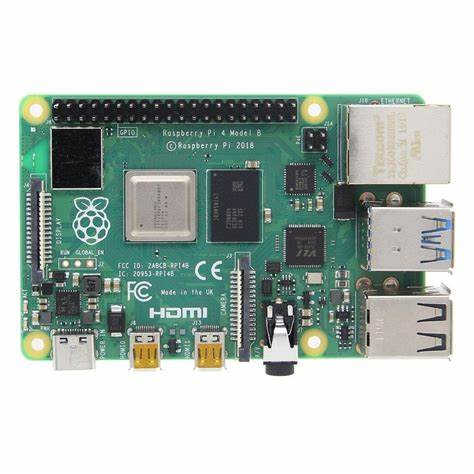
\includegraphics[scale = 0.8]{OIP.jpg}
	\caption{Sensor ultrasonico modelo HC-SR04} 
	\end{center}
	\end{figure}
En las características técnicas tenemos:\\
CPU: Broadcom BCM2711, quad-core Cortex-A72 (ARM v8) 64-bit SoC @ 1.5GHz \\
Memoria RAM: 2GB, 4GB, or 8GB LPDDR4-3200 SDRAM (depende del modelo)\\
Storage: microSD card slot para cargar un SO y archivos\\
Conectividad: Gigabit Ethernet, dual-band 802.11ac wireless, Bluetooth 5.0, Alimentación por USB-C , dos puertos USB 3.0, dos puertos USB 2.0, dos puertos micro-HDMI, 3.5mm audio jack\\
Dimensiones: 88 x 58 x 19.5 mm, 46 g.\\
\begin{figure}[H]
	\begin{center}
	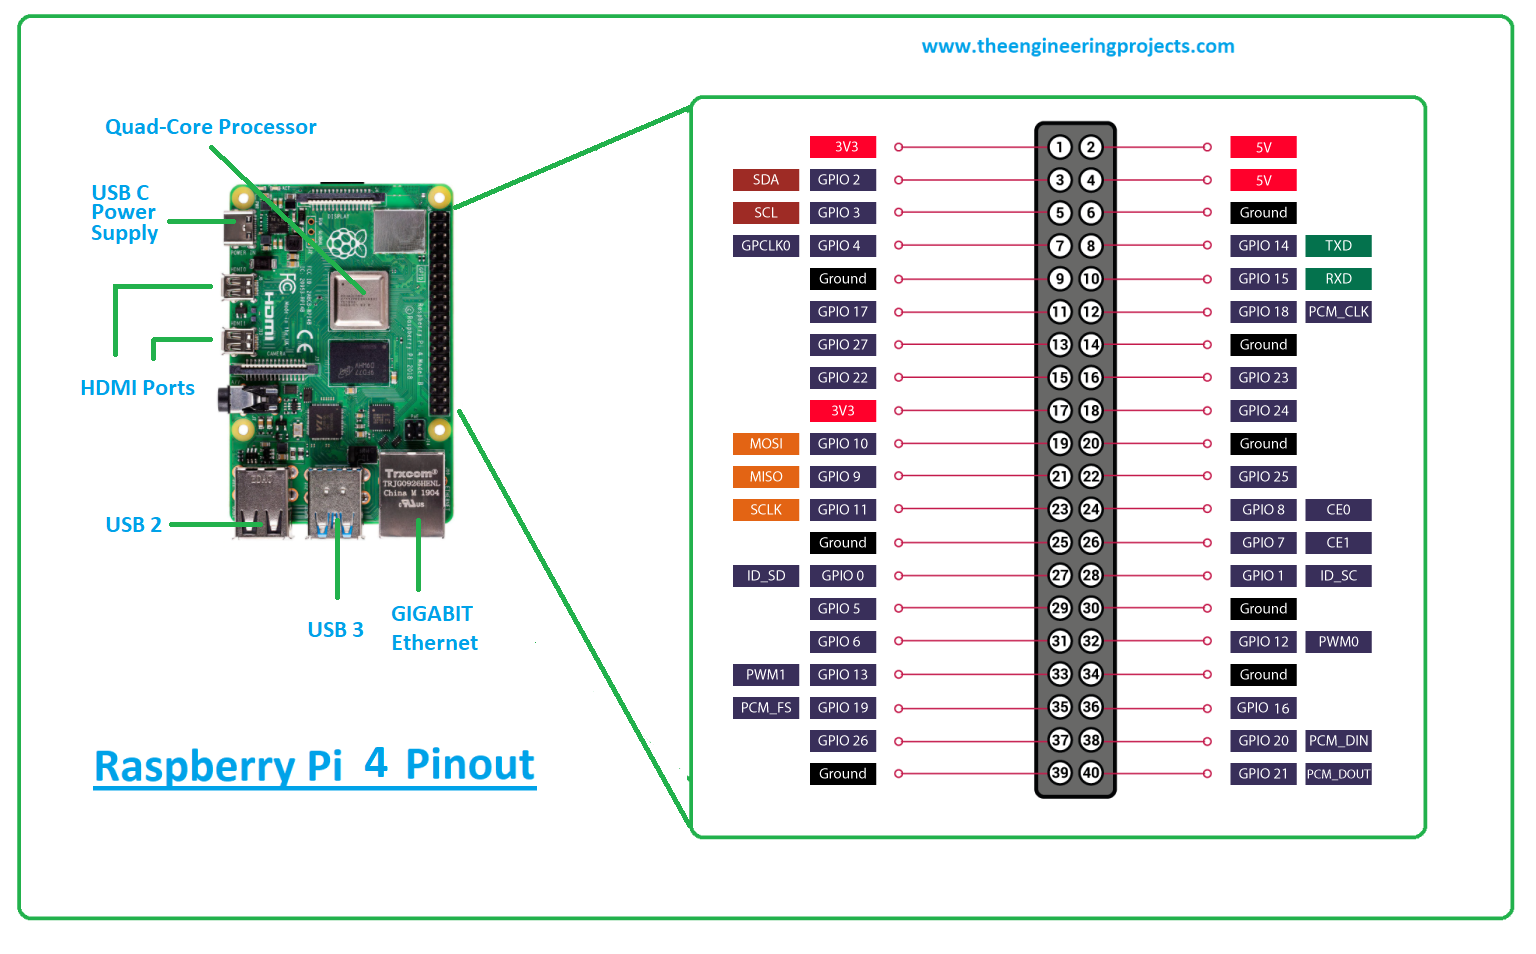
\includegraphics[scale = 0.4]{raspberry-pi-4.jpg}
	\caption{Características del dispositivo Raspberry PI 4 Model B. Imagen disponible en www.raspberrypi.com} 
	\end{center}
	\end{figure}

Este dispositivo cuenta también con 40 GPIOS, que pueden utilizarse de manera conveniente para diferentes propositos. Por otra parte, raspberry UK, proporciona un software llamado Raspberry PI Imager, con el cual se pueden cargar diferentes sistemas operativos compatibles en diferentes versiones, cada una recomendara para las capacidades de memoria RAM correspondientes a cada modelo.

\begin{figure}[H]
	\begin{center}
	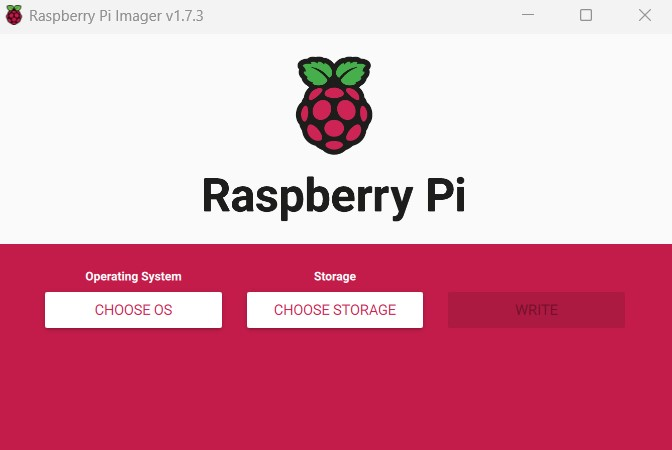
\includegraphics[scale = 0.4]{imager.jpg}
	\caption{Software Imager disponible para Windows y Linux} 
	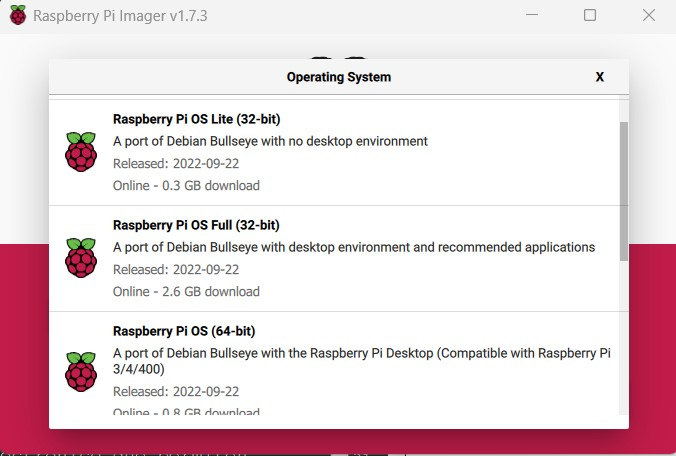
\includegraphics[scale = 0.4]{Imager2.jpg}
	\caption{Sistemas operativos disponibles Raspbian.}
	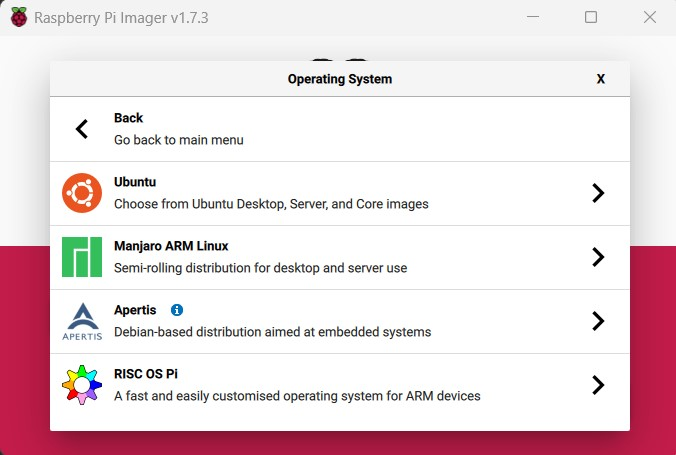
\includegraphics[scale = 0.4]{Imager3.jpg}
	\caption{Sistemas operativos disponibles Linux.}
	\end{center}
	\end{figure}

	\section{Sensores de Distancia}
		\lhead[]{\thesection \ Sensores de Distancia}
Un sensor de distancia es un dispositivo electrónico que permiten obtener el valor de la distancia mediante el uso de ondas ultrasonicas, es decir, hay una onda emitida desde un cabezal, la cual sera reflejada al entrar en contacto con alguna superficie u objeto, tomando lectura de esta misma onda el otro cabezal. Para obtener la distancia se toma como referencia el tiempo de entre la emisión y la recepción de la onda haciendo una conversión de distancia en base en la unidad de segundos que se especifique para cada modelo de sensor. \\
La distancia esta determinada comunmente por:\\
\begin{equation}
L = \dfrac{1}{2} * T * C
\end{equation}
Donde T es el periodo del inverso de los milisegundos entre la emisión y la recepción del sensor y C es una constante correspondiente a la velocidad del sonido que es asociada a: $ C = 343 [m/s]$

%
%\subsection{Sensor Ultrasonico HC-SR04}
%Este modelo de sensor podría considerarse la opción más comercial dentro de los sensores ultrasonicos o sensores de distancia debido a su bajo costo y variedad de aplicaciones con tarjetas de desarrollo y adquisición de datos.
%\begin{figure}[H]
%	\begin{center}
%	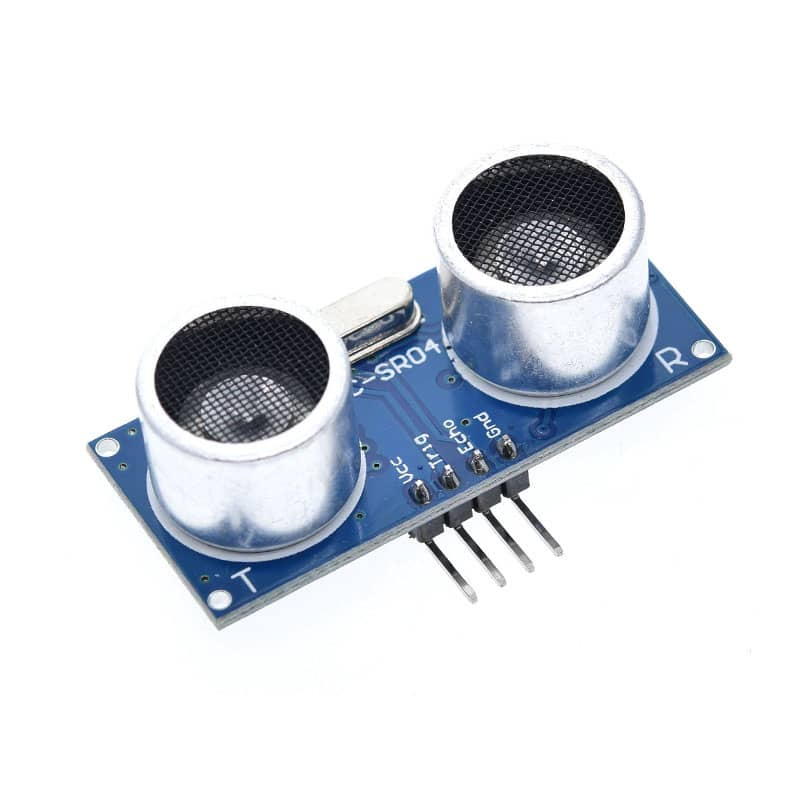
\includegraphics[width =16cm,height =7cm]{HC.jpg}
%	\caption{Sensor ultrasonico modelo HC-SR04} 
%	\end{center}
%	\end{figure}
%	
	
\subsection{Sensor Ultrasonico HC-SRF05}
El sensor ultrasonico HC-SFR05 es un sensor ultrasonico diferente a los modelos HC-SR04, cuya característica principal es que ofrece mayor rango para lecturas y cuenta fisicamente con más pines que son utilizados como pruebas de programación, por lo que generalmente solo se ocupan 4 Pines correspondientes Ground, Vcc, Trigger Pin y Echo Pin.
\begin{figure}[H]
	\begin{center}
	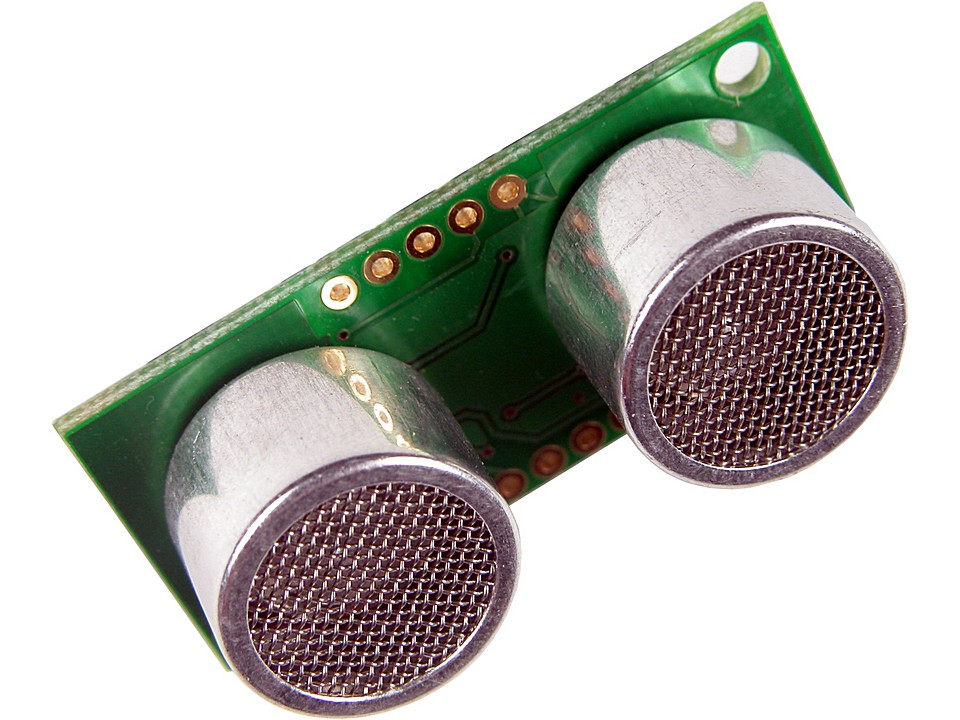
\includegraphics[scale=0.3]{SR.jpg}
	\caption{Sensor ultrasonico modelo HC-SRF05} 
	\end{center}
	\end{figure}
Sus características técnicas son:\\
- Lectura de 1.7 [cm] a 4 [m]\\
- Alimentación de 5 [V] a 4 [mA]\\
- Frecuencia de 40 [KHz]\\

	\section{Sistemas de control de robots móviles}
 	\lhead[]{\thesection \ Sistemas de control de robots móviles}

	\section{ROS}
 	\lhead[]{\thesection \ ROS}
Por sus siglas (Robot Operating System), ROS es un middleware que provee librerías como controladores de dispositivos además de herramientas de visualización y comunicación  para facilitar a los desarrolladores el diseño de software y creación de aplicaciones de robots.\\
ROS tiene compatibilidad con distintos sistemas operativos como Mac OS X, Windows 10, pero principalmente con plataformas basadas en Linux\\
ROS cuenta con distintas distribuciones de diferentes paquetes de ROS, tienen el objetivo de que los programadores trabajen con el código base estable para facilitar la operación de software y hardware. También existen nuevas distribuciones ROS2.\\
Las principales bibliotecas disponibles para cada distribución son:\\
roscpp: Es una biblioteca de cliente C++, a su vez una de las más utilizadas para bibliotecas de alto rendimiento en ROS\\
rospy: Es la biblioteca diseñada para Python del cliente ROS\\
roslip:  Es una biblioteca de cliente LISP y generalmente se utiliza para librerias de planificación.\\


\chapter{METODOLOGÍA} \label{METODOLOGÍA}
 \markboth{METODOLOGÍA}{METODOLOGÍA}

\section{Tren motriz del robot móvil} %\label{Tren motriz del robot móvil}
 \markboth{Tren motriz del robot móvil}{Tren motriz del robot móvil}
 \lhead[]{}


	\section{Protección de la electrónica de potencia}
		\lhead[]{\thesection \ Protección de la electrónica de potencia}
		
		
	\section{Sensores de distancia y retroalimentación
}
		\lhead[]{\thesection \ Sensores de distancia y retroalimentación
}
		
\section{Algoritmo de control móvil} %\label{Algoritmo de control móvil}
 \markboth{Algoritmo de control móvil}{Algoritmo de control móvil}
 \lhead[]{}
\section{Configuración para el controlador Talón SR}
		\lhead[]{\thesection \ Configuración para el controlador Talón SR}
		
Considerando la característica de que la salida de la raspberry tiene una salida de la alimentación de 3.3 V y el rango de la señal de pulso modulada del talon es de 1 a 2 milisegundos, se debe de ajustar el ciclo de trabajo para configurar y calibrar el voltaje de salida para caracterizar los movimientos. De manera similar a la tabla 4.1, ahora tenemos:
\begin{table}[t]
\begin{center}
\begin{tabular}{| p{4cm} | p{3cm} | p{3cm} | p{3cm}  | p{3cm} |} 
	
	\hline
	Movimiento & Voltaje en Rueda 1 & Voltaje en Rueda 2 & Voltaje en Rueda 3 & Voltaje en Rueda 4\\
	\hline
	ALTO & 1.6 & 1.6 & 1.6 & 1.6\\
	\hline
	ADELANTE & 3.3 & 3.3 & 3.3 & 3.3\\
	\hline
	ATRAS & 0.1 & 0.1 & 0.1 & 0.1\\
	\hline
	DERECHA & 3.3 & 0.1 & 0.1 & 3.3\\
	\hline
	IZQUIERDA & 0.1 & 3.3 & 3.3 & 0.1\\
	\hline
	DIAGONAL D1 & 3.3 & 1.6 & 1.6 & 3.3\\
	\hline
	DIAGONAL D2 & 1.6 & 0.1 & 0.1 & 1.6\\
	\hline
	DIAGONAL I1 & 1.6 & 3.3 & 3.3 & 1.6\\
	\hline
	DIAGONAL I2 & 1.6 & 0.1 & 0.1 & 1.6\\
	\hline
Giro en sentido anti horario & 3.3 &3.3 & 0.1 & 0.1\\
	\hline
Giro en sentido horario & 0.1 & 0.1 & 3.3 & 3.3\\
	\hline
\end{tabular}
\caption{Caracterización de movimientos.}
\end{center}
\end{table}
 \section{Diagrama de Flujo para el algoritmo de navegación}
		\lhead[]{\thesection \ Diagrama de Flujo para el algoritmo de navegación} 
		

 \section{Diagramas de conexión}
		\lhead[]{\thesection \ Diagramas de conexión} 
	 \subsection{Propuesta de Diseño del circuito.}
	 En la siguiente figura se muestra la propuesta de los diagramas de conexión del circuito.
	\begin{figure}[H]
	\begin{center}
	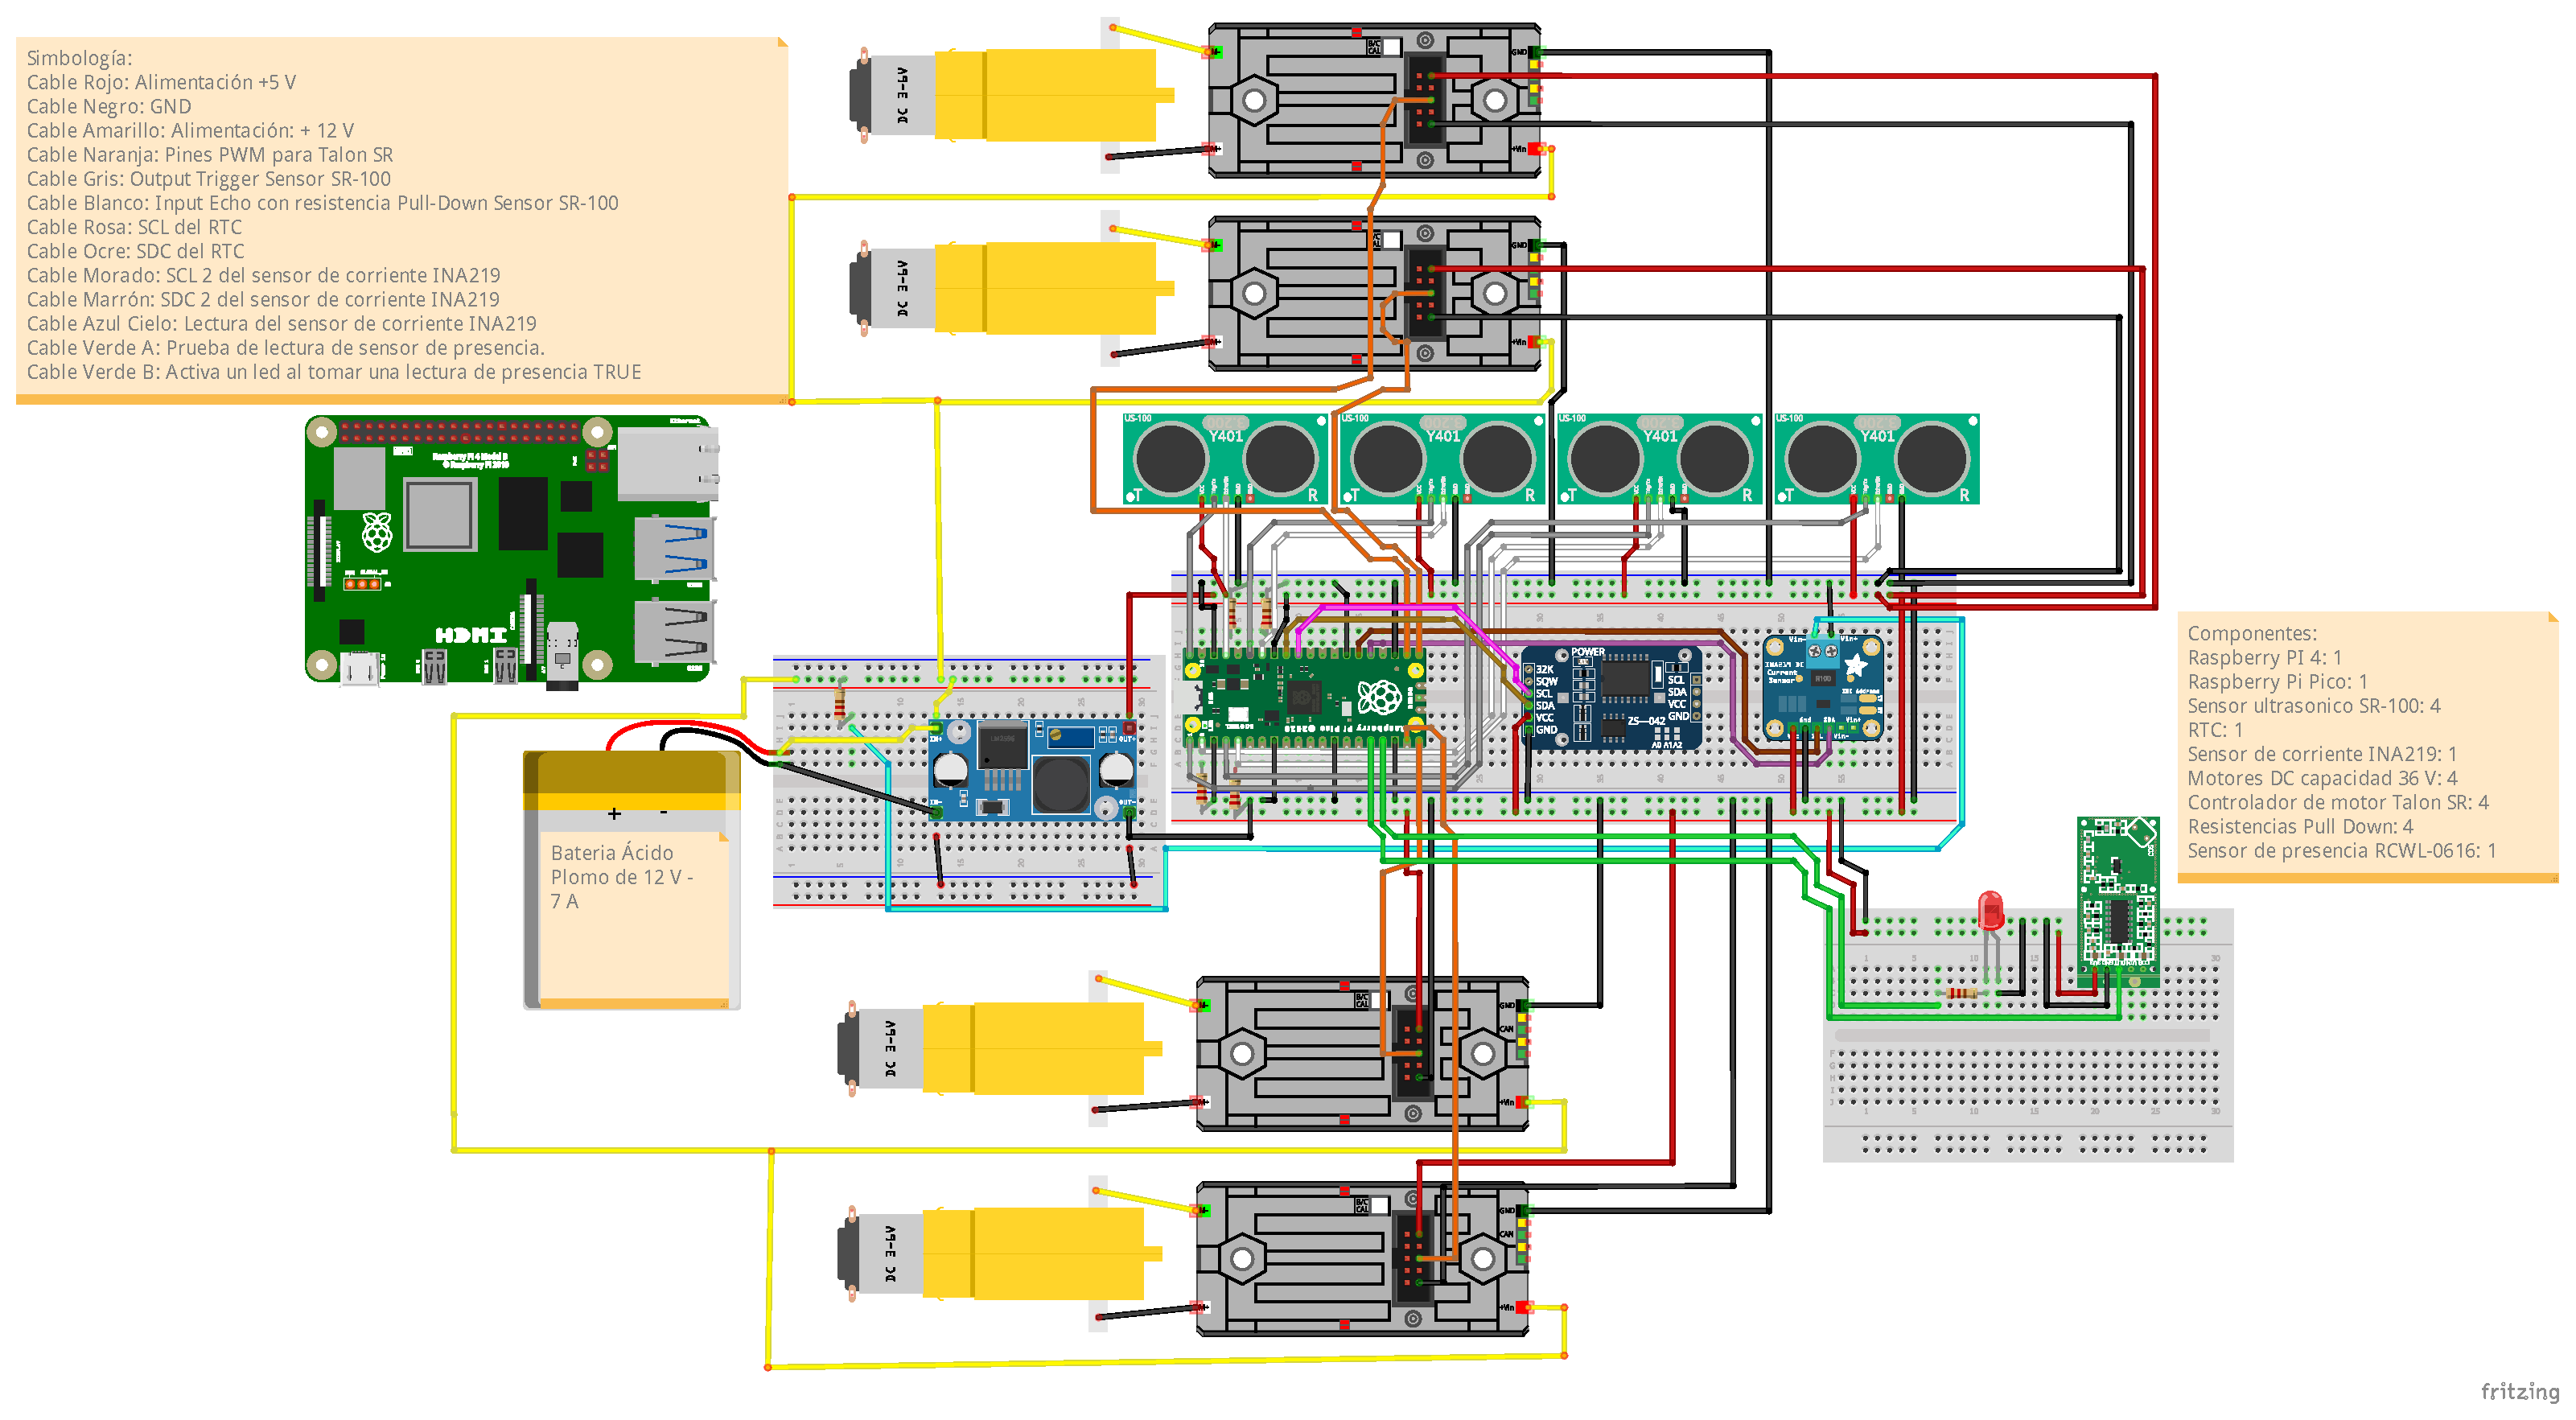
\includegraphics[width =16cm,height =7cm]{Ayudame_Control.pdf}
	\caption{Propuesta de los diagramas de conexión.} 
	\end{center}
	\end{figure}
 
\chapter{Resultados y discusión}
 \markboth{RESULTADOS Y DISCUCIÓN}{RESULTADOS Y DISCUCIÓN}
  \lhead[]{}



\chapter{Conclusiones}
 \markboth{CONCLUSIONES}{CONCLUSIONES}
  \lhead[]{} 


\chapter{Códigos realizados}
 \markboth{Códigos realizados}{Códigos realizados}
  \lhead[]{} 
  
Código de Prueba para un push button.  
\begin{lstlisting}
#include <stdio.h>
#include "pico/stdlib.h"
#include "hardware/gpio.h"

#define BUTTON_PIN 15

int main() {
	stdio_init_all();
	gpio_init(BUTTON_PIN);
	gpio_set_dir(BUTTON_PIN, GPIO_IN);
	gpio_pull_up(BUTTON_PIN);

	while(true) {
		if(!gpio_get(BUTTON_PIN)){
			printf("Button pressed\n");
		}
	sleep_ms(250);
	}
}
\end{lstlisting}

Código Utilizado para un Pin convertidor de lectura análogico Digital y control de encendido de un Led por señal PWM.\\
\begin{lstlisting}
#include <stdio.h>
#include "pico/stdlib.h"
#include "hardware/gpio.h"
#include "hardware/adc.h"
#include "hardware/pwm.h"

#define POT_PIN 26
#define LED_PIN 14

long map(long x, long in_min, long in_max, long out_min, long out_max)
{
	return (x-in_min)*(out_max - out_min) / (in_max - in_min) + out_min;
}

int main()
{
	stdio_init_all();
	adc_init();
	adc_gpio_init(POT_PIN);
	adc_select_input(0);
	gpio_set_function(LED_PIN, GPIO_FUNC_PWM);
	uint slice_num = pwm_gpio_to_slice_num(LED_PIN);
	pwm_set_wrap(slice_num, 255);
	pwm_set_chan_level(slice_num, PWM_CHAN_A, 0);
	pwm_set_enabled(slice_num, true);
	while(1)
	{
		uint16_t result = adc_read();
		long pwm_value = map(result, 0, 4095, 0, 255);
		printf("Raw: %d \t PWM: %d \n", result, pwm_value);
		pwm_set_chan_level(slice_num, PWM_CHAN_A, pwm_value);
		sleep_ms(50);
	}
}

\end{lstlisting}
Código Utilizado para el Display LCD16X02: \\
\begin{lstlisting}
// Programa para Display LCD 16x02 con modulo I2C
// Incluimos las bibliotecas a utilizar
#include <stdio.h>
#include <string.h>
#include "pico/stdlib.h"
#include "hardware/i2c.h"
#include "pico/binary_info.h"

/* Example code to drive a 16x2 LCD panel via a I2C bridge chip (e.g. PCF8574)

   GPIO 4 (pin 6)-> SDA on LCD bridge board
   GPIO 5 (pin 7)-> SCL on LCD bridge board
   5 V (pin 36) -> VCC on LCD bridge board
   GND (pin 38)  -> GND on LCD bridge board
*/
// Comandos
const int LCD_CLEARDISPLAY = 0x01;
const int LCD_RETURNHOME = 0x02;
const int LCD_ENTRYMODESET = 0x04;
const int LCD_DISPLAYCONTROL = 0x08;
const int LCD_CURSORSHIFT = 0x10;
const int LCD_FUNCTIONSET = 0x20;
const int LCD_SETCGRAMADDR = 0x40;
const int LCD_SETDDRAMADDR = 0x80;

// Banderas para entrada del Display
const int LCD_ENTRYSHIFTINCREMENT = 0x01;
const int LCD_ENTRYLEFT = 0x02;

// Banderas para el cursor del Display
const int LCD_BLINKON = 0x01;
const int LCD_CURSORON = 0x02;
const int LCD_DISPLAYON = 0x04;

// flags for display and cursor shift
const int LCD_MOVERIGHT = 0x04;
const int LCD_DISPLAYMOVE = 0x08;

// flags for function set
const int LCD_5x10DOTS = 0x04;
const int LCD_2LINE = 0x08;
const int LCD_8BITMODE = 0x10;

// flag for backlight control
const int LCD_BACKLIGHT = 0x08;
const int LCD_ENABLE_BIT = 0x04;

// By default these LCD display drivers are on bus address 0x27
static int addr = 0x27;

// Modes for lcd_send_byte
#define LCD_CHARACTER  1
#define LCD_COMMAND    0

#define MAX_LINES      2
#define MAX_CHARS      16

/* Quick helper function for single byte transfers */
void i2c_write_byte(uint8_t val) {
#ifdef i2c_default
    i2c_write_blocking(i2c_default, addr, &val, 1, false);
#endif
}

void lcd_toggle_enable(uint8_t val) {
    // Toggle enable pin on LCD display
    // We cannot do this too quickly or things don't work
#define DELAY_US 600
    sleep_us(DELAY_US);
    i2c_write_byte(val | LCD_ENABLE_BIT);
    sleep_us(DELAY_US);
    i2c_write_byte(val & ~LCD_ENABLE_BIT);
    sleep_us(DELAY_US);
}

// The display is sent a byte as two separate nibble transfers
void lcd_send_byte(uint8_t val, int mode) {
    uint8_t high = mode | (val & 0xF0) | LCD_BACKLIGHT;
    uint8_t low = mode | ((val << 4) & 0xF0) | LCD_BACKLIGHT;

    i2c_write_byte(high);
    lcd_toggle_enable(high);
    i2c_write_byte(low);
    lcd_toggle_enable(low);
}

void lcd_clear(void) {
    lcd_send_byte(LCD_CLEARDISPLAY, LCD_COMMAND);
}

// go to location on LCD
void lcd_set_cursor(int line, int position) {
    int val = (line == 0) ? 0x80 + position : 0xC0 + position;
    lcd_send_byte(val, LCD_COMMAND);
}

static void inline lcd_char(char val) {
    lcd_send_byte(val, LCD_CHARACTER);
}

void lcd_string(const char *s) {
    while (*s) {
        lcd_char(*s++);
    }
}

void lcd_init() {
    lcd_send_byte(0x03, LCD_COMMAND);
    lcd_send_byte(0x03, LCD_COMMAND);
    lcd_send_byte(0x03, LCD_COMMAND);
    lcd_send_byte(0x02, LCD_COMMAND);

    lcd_send_byte(LCD_ENTRYMODESET | LCD_ENTRYLEFT, LCD_COMMAND);
    lcd_send_byte(LCD_FUNCTIONSET | LCD_2LINE, LCD_COMMAND);
    lcd_send_byte(LCD_DISPLAYCONTROL | LCD_DISPLAYON, LCD_COMMAND);
    lcd_clear();
}

int main() {
#if !defined(i2c_default) || !defined(PICO_DEFAULT_I2C_SDA_PIN) || !defined(PICO_DEFAULT_I2C_SCL_PIN)
    #warning i2c/lcd_1602_i2c example requires a board with I2C pins
#else
    // This example will use I2C0 on the default SDA and SCL pins (4, 5 on a Pico)
    i2c_init(i2c_default, 100 * 1000);
    gpio_set_function(PICO_DEFAULT_I2C_SDA_PIN, GPIO_FUNC_I2C);
    gpio_set_function(PICO_DEFAULT_I2C_SCL_PIN, GPIO_FUNC_I2C);
    gpio_pull_up(PICO_DEFAULT_I2C_SDA_PIN);
    gpio_pull_up(PICO_DEFAULT_I2C_SCL_PIN);
    // Make the I2C pins available to picotool
    bi_decl(bi_2pins_with_func(PICO_DEFAULT_I2C_SDA_PIN, PICO_DEFAULT_I2C_SCL_PIN, GPIO_FUNC_I2C));

    lcd_init();

    static char *message[] =
            {
                    "Ejemplo LCD16X02", "Raspberry Pi Pico",
            };

    while (1) {
        for (int m = 0; m < sizeof(message) / sizeof(message[0]); m += MAX_LINES) {
            for (int line = 0; line < MAX_LINES; line++) {
                lcd_set_cursor(line, (MAX_CHARS / 2) - strlen(message[m + line]) / 2);
                lcd_string(message[m + line]);
            }
            sleep_ms(2000);
            lcd_clear();
        }
    }

    return 0;
#endif
}

\end{lstlisting}

Código Utilizado para Calibrar el Talon SR:\\

\begin{lstlisting}
//incluimos todas las bibliotecas que vamos a usar con las funciones para PWM, ADC y GPIO
#include <stdio.h>
#include "pico/stdlib.h"
#include "hardware/gpio.h"
#include "hardware/adc.h"
#include "hardware/pwm.h"

//Definimos los nombres de los GPIO que vamos a usar
#define POT_PIN 26
#define LED_PIN 14
#define CAL_PIN 15 // Este pin se usara para calibrar el Talon


//EL PWM utiliza el reloj del sistema, cada pulso tiene una frecuencia de 125 MHz es decir 8 nano segundos de tiempo, si queremos que
//el TALON SR funcione debemos tener una frecuencia de 1-2 ms con este valor sabremos cual es el valor maximo de ciclos que queremos contar para el PWM
//Si seleccionamos 2 ms como frecuencia el numero de ciclos es: 2ms/8ns = 250,000. pero el PWM llega hasta 65535 por lo que por default se tiene una frecuencia minima de 1.9KHz.
//Por esta razon debemos usar el divider de PWM si queremos 633Hz que es un periodo de 1.66ms entonces el divider es 1.9kHz/3 = 633Hz, divider = 3
//Divider = (125000000/(4096*frecuenciaDeseada))/16



    //existen 8 slices para el PWM cada slice tiene dos salidas PWM, 
    //en total hay 16 salidas PWM, y todos los GPIO pueden controlarlos
    //Para el GPIO 14 es el PWM_A_7, Para el GPIO 15 ES EL PWM_A_B
    


// creamos una funcion para que funcione el pwm desde 0 a 180



//El ADC es de 12 bits por lo que el maximo valor es de 4095
long map(long x, long in_min, long in_max, long out_min, long out_max)
{
    return (x - in_min)*(out_max-out_min) / (in_max-in_min) + out_min;
}

int main(){
    
    
    int frecuenciaDeseada = 300;
    float Divider = (125000000/(4096*frecuenciaDeseada))/16; //= 3.81
    
    long ciclos =  65535;//numero de ciclos del wrap y numero de ciclos maximo del contador

    //iniciamos la biblioteca stdio para que funcione todo el programa
    stdio_init_all();

    //Le damos reloj al ADCA	
    adc_init();
//-------------------- INICIALIZACION ADC-------------------------------
    adc_gpio_init(POT_PIN);//iniciamos el PIN 26 correspondiente al ADC que lee el potenciometro
    adc_select_input(0);//Activamos el canal 0 del ADC para el potenciometro
    //canal 0 corresponde a pin 26
    //canal 1 corresponde a pin 27
    //canal 2 corresponde a pin 28
    //canal 3 corresponde a pin 29, aqui se encuentra el sensor de temperatura
    
//-------------------- INICIALIZACION PWM LED---------------------------
    gpio_set_function(LED_PIN, GPIO_FUNC_PWM); // seleccionamos la funcion de gpio con el 
    //numero de pin correspondiente a LED_PIN, la funcion sera PWM
    
//-------------------- INICIALIZACION PWM TALON----------------------------------------
    gpio_set_function(CAL_PIN, GPIO_FUNC_PWM); // seleccionamos la funcion de gpio con el 
    //numero de pin correspondiente a CAL_PIN, la funcion sera PWM

    //LO de abajo significa que seleccionamos el PWM 7, ambos canales A y B
    uint slice_num = pwm_gpio_to_slice_num(LED_PIN);
    
    //Utilizamos la funcion que dividira el reloj del sistema
    pwm_set_clkdiv (slice_num, Divider);

    //"ciclos" es el valor maximo antes de reiniciar el contador a 0
    pwm_set_wrap(slice_num, ciclos);

    pwm_set_chan_level(slice_num, PWM_CHAN_A,0); //Empezamos en 0 el nivel del PWM
    //RECORDEMOS QUE ESTAMOS EN EL CANAL A
    pwm_set_chan_level(slice_num, PWM_CHAN_B,0); //Empezamos en 0 el nivel del PWM
    //RECORDEMOS QUE ESTAMOS EN EL CANAL B

    pwm_set_enabled(slice_num,true); //Habilitamos el PWM

//loop principal
    while (1)
    {
         uint16_t result = adc_read(); //Leemos el resultado del ADC del potenciometro

         long pwm_value = map(result, 0, 4095, 0, ciclos); //convertimos el resultado del potenciometro a un valor entre 0 a ciclos
         
         float voltaje = pwm_value*3.3/65635;

         printf("Raw: %d \t PWM: %d \t Voltaje PWM: %.1f \n", result, pwm_value, voltaje);
        //imprimimos el valor del resultado del ADC y el valor para el PWM 
        //para visualizar valores en pantalla usamos sudo minicom -b 115200 -o -D /dev/ttyACM0


        //SELECCIONAMOS CON PWM_VALUE LA CANTIDAD DE CICLOS QUE QUEREMOS 
        //EN ALTO DENTRO DEL PERIODO DE 180, EJ, SI pwm_value ES 10 PUES 10 CICLOS DE LOS 
        //180 SERAN 1, LOS DEMAS SERAN 0

        //INDICAMOS QUE USAREMOS EL NUMERO DE SLICE 7 PORQUE LO DECLARAMOS ARRIBA
        
        //INDICAMOS QUE USAREMOS EL CANAL A
        //INDICAMOS QUE USAMOS EL VALOR DEL PWM DEL POTENCIOMETRO
         pwm_set_chan_level(slice_num, PWM_CHAN_A, pwm_value);
         
        //INDICAMOS QUE USAREMOS EL CANAL B
        //INDICAMOS QUE USAMOS EL VALOR DEL PWM DEL POTENCIOMETRO
         pwm_set_chan_level(slice_num, PWM_CHAN_B, pwm_value);
         
         
         //RETARDO DE 50ms para visualizar los datos en la pantalla
         sleep_ms(100);
    }
    
}

\end{lstlisting}


Código Utilizado para los sensores Ultrasónicos:\\
\begin{lstlisting}
// Programa de sensor ultrasonico
// INcluimos las librerias a utilizar

#include <stdio.h>
#include "pico/stdlib.h"
#include "hardware/gpio.h"
// Definios los GPIOS
uint trigPin=2;
uint echoPin=3;

// definimos un tiempo de salida 
int timeout = 26100;
// Definimos una funcion para inicializar los Gpios
void setupUltrasonicPins(uint trigPin, uint echoPin)
{
	gpio_init(trigPin);
	gpio_init(echoPin);
	gpio_set_dir(trigPin, GPIO_OUT);
	gpio_set_dir(echoPin, GPIO_IN);
}
// uint64
uint64_t getPulse(uint trigPin, uint echoPin)
{
	gpio_put(trigPin, 1);
	sleep_us(10);
	gpio_put(trigPin, 0);
	uint width = 0;
	while(gpio_get(echoPin) == 0) tight_loop_contents();
	while(gpio_get(echoPin) == 1)
	{
		width++;
		sleep_us(1);
		if(width > timeout) return 0;
	}
	return width;
}
int getCm(uint trigPin, uint echoPin)
{
	uint64_t pulseLength = getPulse(trigPin, echoPin);
	return pulseLength / 29 / 2;
}
int getInch (uint trigPin, uint echoPin)
{
	uint64_t pulseLength = getPulse(trigPin, echoPin);
	return (long)pulseLength /74.f /2.f;
}
// Definimos la funcion principal
int main()
{
	stdio_init_all();
	setupUltrasonicPins(trigPin, echoPin);

	while(true)
	{

		if (getCm(trigPin, echoPin) <= 6){
			printf("\n Distancia minima: \t  %d \t cm \t Alto", getCm(trigPin, echoPin));
			sleep_ms(500);
		}
		else if (getCm(trigPin, echoPin) >= 7  && getCm(trigPin, echoPin) <= 15){
			printf("\n Distancia cercana: \t %d \t  cm  \t Girar", getCm(trigPin, echoPin));
			sleep_ms(500);
		}
		else if (16 <= getCm(trigPin, echoPin)){
			printf("\n Distancia Segura: \t %d \t cm \t Avanzar", getCm(trigPin, echoPin));
			sleep_ms(500);
		}


	}
}

\end{lstlisting}
    
 %falta completa con la información babababbab
	
	%La bibliografia se incluye en el formato preferido, automaticamente se numera, debemos de agregar
	%una etiqueta al principio para pode hacer una referencia después
	
\begin{thebibliography}{} 
 \addcontentsline{toc}{chapter}{Bibliografía}

%%%%%%%%%%%%%%%%%%%%%%%%%%%%%%%%%%%%%%%%%%%%%%%%%%%%%%%%%%%%%%%%%%%%%%%%%%%%%%%%%%%%%%%%%%%%%
%%%%%%%%%%%%%%%%%%%%%%%%%%%%%%%CITAS DE LOS ANTECEDENTES%%%%%%%%%%%%%%%%%%%%%%%%%%%%%%%%%%%%%
%%%%%%%%%%%%%%%%%%%%%%%%%%%%%%%%%%%%%%%%%%%%%%%%%%%%%%%%%%%%%%%%%%%%%%%%%%%%%%%%%%%%%%%%%%%%%
	
	\bibitem{WHO}  WHO, “WHO Coronavirus Disease (COVID-19) Dashboard”. [En línea]. Disponible en:\\ $https://covid19.who.int/$.

	\bibitem {Unautor} “Covid-19 México, Datos Abiertos Dirección General de Epidemiología”.  [En línea]. Disponible en:\\ $https://datos.covid-19.conacyt.mx/$

	
	\bibitem {Igoe} M. Igoe y V. Chadwick, “After the pandemic : How will COVID-19 transform global health and development ?”, Devex, núm. April, pp. 1–9, 2020.

	
	\bibitem {Barrie} V. M. Lomas-Barrié, M. Peña-Cabrera, y T. Alcantara-Concepcion, “AYUDAME 1.0”, 2020. [En línea]. Disponible en:\\ $http://www.leai4.iimas.unam.mx/?page_id=101. [Consultado: 07-jul-2020].$
	
	\bibitem {Durrant} H. Durrant-Whyte y T. Bailey, “Simultaneous localization and mapping: Part I”, IEEE Robot. Autom. Mag., vol. 13, núm. 2, pp. 99–108, 2006. 
	
	\bibitem {Bailey} Bailey y H. Durrant-Whyte, “Simultaneous localization and mapping (SLAM): Part II”, IEEE Robot. Autom. Mag., vol. 13, núm. 3, pp. 108–117, 2006.
	
	\bibitem {Gatesichapakorn} S. Gatesichapakorn, J. Takamatsu, y M. Ruchanurucks, “ROS based Autonomous Mobile Robot Navigation using 2D LiDAR and RGB-D Camera”, 2019 1st Int. Symp. Instrumentation, Control. Artif. Intell. Robot. ICA-SYMP 2019, pp. 151–154, 2019.
	
	\bibitem {Liu} R. Liu, J. Shen, C. Chen, y J. Yang, “SLAM for Robotic Navigation by Fusing RGB-D and Inertial Data in Recurrent and Convolutional Neural Networks”, 2019 IEEE 5th Int. Conf.
Mechatronics Syst. Robot. ICMSR 2019, pp. 1–6, 2019.

	\bibitem {Henry} P. Henry, M. Krainin, E. Herbst, X. Ren, y D. Fox, “RGB-D mapping: Using depth cameras forense 3D modeling of indoor environments”, en Springer Tracts in Advanced Robotics, 2014, vol. 79, pp. 477–491.
	
	\bibitem {Endres} F. Endres, J. Hess, J. Sturm, D. Cremers, y W. Burgard, “3-D Mapping with an RGB-D camera”, en IEEE Transactions on Robotics, 2014, vol. 30, núm. 1, pp. 177–187.
	
	\bibitem {Labbé} M. Labbé y F. Michaud, “Online global loop closure detection for large-scale multi-session graph-based SLAM”, en IEEE International Conference on Intelligent Robots and Systems, 2014, pp. 2661–2666.
	
	\bibitem  {Guo} X. Liu, B. Guo, y C. Meng, “A method of simultaneous location and mapping based on RGB-D cameras”, en 2016 14th International Conference on Control, Automation, Robotics and Vision, ICARCV 2016, 2017.
	
	\bibitem {Barrie} V. Lomas-Barrie, M. Peña-Cabrera, y J. Durán-Ortega, “Determining humanoid soccer player position based on Goal detection”, en Proceedings of the 2015 International Conference on Artificial Intelligence, ICAI 2015 - WORLDCOMP 2015, 2015, pp. 61–65.

	
	\bibitem {Mario} P.-C. Mario, L.-J. Ismael, R.-C. Reyes, y C.-C. Jorge, “Machine vision approach for robotic assembly”, Assem. Autom., vol. 25, núm. 3, pp. 204–216, 2005.

	\bibitem {IFR} IFR Press Release. Industrial Robots: Robot Investment Reaches Record 16.5 billion USD. Shanghai, Frankfurt, Sep 18, 2019 [consultado 9 Mar 2019] Disponible en: https://ifr.org/ifr-press-releases/news/robot-investment-reaches-record-16.5-billion-usd

	\bibitem {Posibilidades} Posibilidades de la robótica y perspectivas de la robótica en la medicina https://www.revistadyna.com/busqueda/posibilidades-y-perspectivas-de-robotica-en-medicina
	
	\bibitem {Ramos} Ramos, A. C. (2001). Estado del arte en cirugía robótica. Revista Mexicana de Cirugía Endoscópica, 2(2), 109 112.
	
	\bibitem {Cornejo} Cornejo Aguilar, J. A., Cornejo, J., Vargas, M.,  Sebastian , R. (2019). La revolución de la cirugía robótica en latino américa y la futura implementación en el sistema de salud del Per ú. Revista de la Facultad de Medicina Humana, 19(1), 16. 16.[10] R.H. Taylor A Perspective on Medical Robotics Proceedings of the IEEE., 
	
\end{thebibliography}

\end{document}